% Options for packages loaded elsewhere
\PassOptionsToPackage{unicode}{hyperref}
\PassOptionsToPackage{hyphens}{url}
%
\documentclass[
]{article}
\usepackage{lmodern}
\usepackage{amssymb,amsmath}
\usepackage{ifxetex,ifluatex}
\ifnum 0\ifxetex 1\fi\ifluatex 1\fi=0 % if pdftex
  \usepackage[T1]{fontenc}
  \usepackage[utf8]{inputenc}
  \usepackage{textcomp} % provide euro and other symbols
\else % if luatex or xetex
  \usepackage{unicode-math}
  \defaultfontfeatures{Scale=MatchLowercase}
  \defaultfontfeatures[\rmfamily]{Ligatures=TeX,Scale=1}
\fi
% Use upquote if available, for straight quotes in verbatim environments
\IfFileExists{upquote.sty}{\usepackage{upquote}}{}
\IfFileExists{microtype.sty}{% use microtype if available
  \usepackage[]{microtype}
  \UseMicrotypeSet[protrusion]{basicmath} % disable protrusion for tt fonts
}{}
\makeatletter
\@ifundefined{KOMAClassName}{% if non-KOMA class
  \IfFileExists{parskip.sty}{%
    \usepackage{parskip}
  }{% else
    \setlength{\parindent}{0pt}
    \setlength{\parskip}{6pt plus 2pt minus 1pt}}
}{% if KOMA class
  \KOMAoptions{parskip=half}}
\makeatother
\usepackage{xcolor}
\IfFileExists{xurl.sty}{\usepackage{xurl}}{} % add URL line breaks if available
\IfFileExists{bookmark.sty}{\usepackage{bookmark}}{\usepackage{hyperref}}
\hypersetup{
  pdftitle={Casestudy2DDS},
  pdfauthor={Dylan Scott},
  hidelinks,
  pdfcreator={LaTeX via pandoc}}
\urlstyle{same} % disable monospaced font for URLs
\usepackage[margin=1in]{geometry}
\usepackage{color}
\usepackage{fancyvrb}
\newcommand{\VerbBar}{|}
\newcommand{\VERB}{\Verb[commandchars=\\\{\}]}
\DefineVerbatimEnvironment{Highlighting}{Verbatim}{commandchars=\\\{\}}
% Add ',fontsize=\small' for more characters per line
\usepackage{framed}
\definecolor{shadecolor}{RGB}{248,248,248}
\newenvironment{Shaded}{\begin{snugshade}}{\end{snugshade}}
\newcommand{\AlertTok}[1]{\textcolor[rgb]{0.94,0.16,0.16}{#1}}
\newcommand{\AnnotationTok}[1]{\textcolor[rgb]{0.56,0.35,0.01}{\textbf{\textit{#1}}}}
\newcommand{\AttributeTok}[1]{\textcolor[rgb]{0.77,0.63,0.00}{#1}}
\newcommand{\BaseNTok}[1]{\textcolor[rgb]{0.00,0.00,0.81}{#1}}
\newcommand{\BuiltInTok}[1]{#1}
\newcommand{\CharTok}[1]{\textcolor[rgb]{0.31,0.60,0.02}{#1}}
\newcommand{\CommentTok}[1]{\textcolor[rgb]{0.56,0.35,0.01}{\textit{#1}}}
\newcommand{\CommentVarTok}[1]{\textcolor[rgb]{0.56,0.35,0.01}{\textbf{\textit{#1}}}}
\newcommand{\ConstantTok}[1]{\textcolor[rgb]{0.00,0.00,0.00}{#1}}
\newcommand{\ControlFlowTok}[1]{\textcolor[rgb]{0.13,0.29,0.53}{\textbf{#1}}}
\newcommand{\DataTypeTok}[1]{\textcolor[rgb]{0.13,0.29,0.53}{#1}}
\newcommand{\DecValTok}[1]{\textcolor[rgb]{0.00,0.00,0.81}{#1}}
\newcommand{\DocumentationTok}[1]{\textcolor[rgb]{0.56,0.35,0.01}{\textbf{\textit{#1}}}}
\newcommand{\ErrorTok}[1]{\textcolor[rgb]{0.64,0.00,0.00}{\textbf{#1}}}
\newcommand{\ExtensionTok}[1]{#1}
\newcommand{\FloatTok}[1]{\textcolor[rgb]{0.00,0.00,0.81}{#1}}
\newcommand{\FunctionTok}[1]{\textcolor[rgb]{0.00,0.00,0.00}{#1}}
\newcommand{\ImportTok}[1]{#1}
\newcommand{\InformationTok}[1]{\textcolor[rgb]{0.56,0.35,0.01}{\textbf{\textit{#1}}}}
\newcommand{\KeywordTok}[1]{\textcolor[rgb]{0.13,0.29,0.53}{\textbf{#1}}}
\newcommand{\NormalTok}[1]{#1}
\newcommand{\OperatorTok}[1]{\textcolor[rgb]{0.81,0.36,0.00}{\textbf{#1}}}
\newcommand{\OtherTok}[1]{\textcolor[rgb]{0.56,0.35,0.01}{#1}}
\newcommand{\PreprocessorTok}[1]{\textcolor[rgb]{0.56,0.35,0.01}{\textit{#1}}}
\newcommand{\RegionMarkerTok}[1]{#1}
\newcommand{\SpecialCharTok}[1]{\textcolor[rgb]{0.00,0.00,0.00}{#1}}
\newcommand{\SpecialStringTok}[1]{\textcolor[rgb]{0.31,0.60,0.02}{#1}}
\newcommand{\StringTok}[1]{\textcolor[rgb]{0.31,0.60,0.02}{#1}}
\newcommand{\VariableTok}[1]{\textcolor[rgb]{0.00,0.00,0.00}{#1}}
\newcommand{\VerbatimStringTok}[1]{\textcolor[rgb]{0.31,0.60,0.02}{#1}}
\newcommand{\WarningTok}[1]{\textcolor[rgb]{0.56,0.35,0.01}{\textbf{\textit{#1}}}}
\usepackage{graphicx,grffile}
\makeatletter
\def\maxwidth{\ifdim\Gin@nat@width>\linewidth\linewidth\else\Gin@nat@width\fi}
\def\maxheight{\ifdim\Gin@nat@height>\textheight\textheight\else\Gin@nat@height\fi}
\makeatother
% Scale images if necessary, so that they will not overflow the page
% margins by default, and it is still possible to overwrite the defaults
% using explicit options in \includegraphics[width, height, ...]{}
\setkeys{Gin}{width=\maxwidth,height=\maxheight,keepaspectratio}
% Set default figure placement to htbp
\makeatletter
\def\fps@figure{htbp}
\makeatother
\setlength{\emergencystretch}{3em} % prevent overfull lines
\providecommand{\tightlist}{%
  \setlength{\itemsep}{0pt}\setlength{\parskip}{0pt}}
\setcounter{secnumdepth}{-\maxdimen} % remove section numbering
\usepackage{amsmath}
\usepackage{booktabs}
\usepackage{caption}
\usepackage{longtable}

\title{Casestudy2DDS}
\author{Dylan Scott}
\date{4/6/2021}

\begin{document}
\maketitle

\hypertarget{youtube-link}{%
\subsection{Youtube link}\label{youtube-link}}

Dylan's Case study 2 Video

\hypertarget{project-overview}{%
\subsection{Project Overview}\label{project-overview}}

\hypertarget{data-breakdown}{%
\subsection{Data Breakdown}\label{data-breakdown}}

870 observation with 36 variables

\begin{Shaded}
\begin{Highlighting}[]
\KeywordTok{library}\NormalTok{(knitr)}
\KeywordTok{library}\NormalTok{(tidyverse)}
\KeywordTok{library}\NormalTok{(readxl)}
\KeywordTok{library}\NormalTok{(curl)}
\KeywordTok{library}\NormalTok{(GGally)}
\KeywordTok{library}\NormalTok{(e1071)}
\KeywordTok{library}\NormalTok{(caret)}
\KeywordTok{library}\NormalTok{(ggcorrplot)}
\KeywordTok{library}\NormalTok{(gridExtra)}
\KeywordTok{library}\NormalTok{(reticulate)}
\KeywordTok{library}\NormalTok{(gt)}


\NormalTok{data <-}\KeywordTok{read.csv}\NormalTok{(}\KeywordTok{curl}\NormalTok{(}\StringTok{"https://raw.githubusercontent.com/Scottdyl/CaseStudy2DDS/main/data/CaseStudy2-data.csv"}\NormalTok{))}

\CommentTok{#summary(data)}
\CommentTok{#no missing values found}

\CommentTok{#convert raw data variables to factors}
\NormalTok{data}\OperatorTok{$}\NormalTok{Education =}\StringTok{ }\KeywordTok{as.factor}\NormalTok{(data}\OperatorTok{$}\NormalTok{Education)}
\NormalTok{data}\OperatorTok{$}\NormalTok{EnvironmentSatisfaction =}\StringTok{ }\KeywordTok{as.factor}\NormalTok{(data}\OperatorTok{$}\NormalTok{EnvironmentSatisfaction)}
\NormalTok{data}\OperatorTok{$}\NormalTok{JobInvolvement =}\StringTok{ }\KeywordTok{as.factor}\NormalTok{(data}\OperatorTok{$}\NormalTok{JobInvolvement)}
\NormalTok{data}\OperatorTok{$}\NormalTok{JobLevel =}\StringTok{ }\KeywordTok{as.factor}\NormalTok{(data}\OperatorTok{$}\NormalTok{JobLevel)}
\NormalTok{data}\OperatorTok{$}\NormalTok{JobSatisfaction =}\StringTok{ }\KeywordTok{as.factor}\NormalTok{(data}\OperatorTok{$}\NormalTok{JobSatisfaction)}
\NormalTok{data}\OperatorTok{$}\NormalTok{PerformanceRating =}\StringTok{ }\KeywordTok{as.factor}\NormalTok{(data}\OperatorTok{$}\NormalTok{PerformanceRating)}
\NormalTok{data}\OperatorTok{$}\NormalTok{RelationshipSatisfaction =}\StringTok{ }\KeywordTok{as.factor}\NormalTok{(data}\OperatorTok{$}\NormalTok{RelationshipSatisfaction)}
\NormalTok{data}\OperatorTok{$}\NormalTok{WorkLifeBalance =}\StringTok{ }\KeywordTok{as.factor}\NormalTok{(data}\OperatorTok{$}\NormalTok{WorkLifeBalance)}


\CommentTok{# no attr data}
\NormalTok{Comp_attr <-}\StringTok{ }\KeywordTok{read.csv}\NormalTok{(}\KeywordTok{curl}\NormalTok{(}\StringTok{"https://raw.githubusercontent.com/Scottdyl/CaseStudy2DDS/main/data/CaseStudy2CompSet%20No%20Attrition.csv"}\NormalTok{))}
\NormalTok{Comp_attr}\OperatorTok{$}\NormalTok{Education =}\StringTok{ }\KeywordTok{as.factor}\NormalTok{(Comp_attr}\OperatorTok{$}\NormalTok{Education)}
\NormalTok{Comp_attr}\OperatorTok{$}\NormalTok{EnvironmentSatisfaction =}\StringTok{ }\KeywordTok{as.factor}\NormalTok{(Comp_attr}\OperatorTok{$}\NormalTok{EnvironmentSatisfaction)}
\NormalTok{Comp_attr}\OperatorTok{$}\NormalTok{JobInvolvement =}\StringTok{ }\KeywordTok{as.factor}\NormalTok{(Comp_attr}\OperatorTok{$}\NormalTok{JobInvolvement)}
\NormalTok{Comp_attr}\OperatorTok{$}\NormalTok{JobLevel =}\StringTok{ }\KeywordTok{as.factor}\NormalTok{(Comp_attr}\OperatorTok{$}\NormalTok{JobLevel)}
\NormalTok{Comp_attr}\OperatorTok{$}\NormalTok{JobSatisfaction =}\StringTok{ }\KeywordTok{as.factor}\NormalTok{(Comp_attr}\OperatorTok{$}\NormalTok{JobSatisfaction)}
\NormalTok{Comp_attr}\OperatorTok{$}\NormalTok{PerformanceRating =}\StringTok{ }\KeywordTok{as.factor}\NormalTok{(Comp_attr}\OperatorTok{$}\NormalTok{PerformanceRating)}
\NormalTok{Comp_attr}\OperatorTok{$}\NormalTok{RelationshipSatisfaction =}\StringTok{ }\KeywordTok{as.factor}\NormalTok{(Comp_attr}\OperatorTok{$}\NormalTok{RelationshipSatisfaction)}
\NormalTok{Comp_attr}\OperatorTok{$}\NormalTok{WorkLifeBalance =}\StringTok{ }\KeywordTok{as.factor}\NormalTok{(Comp_attr}\OperatorTok{$}\NormalTok{WorkLifeBalance)}


\CommentTok{# no sal data}
\NormalTok{Comp_sal <-}\KeywordTok{read.csv}\NormalTok{(}\KeywordTok{curl}\NormalTok{(}\StringTok{"https://raw.githubusercontent.com/Scottdyl/CaseStudy2DDS/main/data/CaseStudy2CompSet%20No%20Salary.csv"}\NormalTok{))}
\NormalTok{Comp_sal}\OperatorTok{$}\NormalTok{Education =}\StringTok{ }\KeywordTok{as.factor}\NormalTok{(Comp_sal}\OperatorTok{$}\NormalTok{Education)}
\NormalTok{Comp_sal}\OperatorTok{$}\NormalTok{EnvironmentSatisfaction =}\StringTok{ }\KeywordTok{as.factor}\NormalTok{(Comp_sal}\OperatorTok{$}\NormalTok{EnvironmentSatisfaction)}
\NormalTok{Comp_sal}\OperatorTok{$}\NormalTok{JobInvolvement =}\StringTok{ }\KeywordTok{as.factor}\NormalTok{(Comp_sal}\OperatorTok{$}\NormalTok{JobInvolvement)}
\NormalTok{Comp_sal}\OperatorTok{$}\NormalTok{JobLevel =}\StringTok{ }\KeywordTok{as.factor}\NormalTok{(Comp_sal}\OperatorTok{$}\NormalTok{JobLevel)}
\NormalTok{Comp_sal}\OperatorTok{$}\NormalTok{JobSatisfaction =}\StringTok{ }\KeywordTok{as.factor}\NormalTok{(Comp_sal}\OperatorTok{$}\NormalTok{JobSatisfaction)}
\NormalTok{Comp_sal}\OperatorTok{$}\NormalTok{PerformanceRating =}\StringTok{ }\KeywordTok{as.factor}\NormalTok{(Comp_sal}\OperatorTok{$}\NormalTok{PerformanceRating)}
\NormalTok{Comp_sal}\OperatorTok{$}\NormalTok{RelationshipSatisfaction =}\StringTok{ }\KeywordTok{as.factor}\NormalTok{(Comp_sal}\OperatorTok{$}\NormalTok{RelationshipSatisfaction)}
\NormalTok{Comp_sal}\OperatorTok{$}\NormalTok{WorkLifeBalance =}\StringTok{ }\KeywordTok{as.factor}\NormalTok{(Comp_sal}\OperatorTok{$}\NormalTok{WorkLifeBalance)}

\KeywordTok{head}\NormalTok{(data)}
\end{Highlighting}
\end{Shaded}

\begin{verbatim}
##   ID Age Attrition    BusinessTravel DailyRate             Department DistanceFromHome Education   EducationField
## 1  1  32        No     Travel_Rarely       117                  Sales               13         4    Life Sciences
## 2  2  40        No     Travel_Rarely      1308 Research & Development               14         3          Medical
## 3  3  35        No Travel_Frequently       200 Research & Development               18         2    Life Sciences
## 4  4  32        No     Travel_Rarely       801                  Sales                1         4        Marketing
## 5  5  24        No Travel_Frequently       567 Research & Development                2         1 Technical Degree
## 6  6  27        No Travel_Frequently       294 Research & Development               10         2    Life Sciences
##   EmployeeCount EmployeeNumber EnvironmentSatisfaction Gender HourlyRate JobInvolvement JobLevel
## 1             1            859                       2   Male         73              3        2
## 2             1           1128                       3   Male         44              2        5
## 3             1           1412                       3   Male         60              3        3
## 4             1           2016                       3 Female         48              3        3
## 5             1           1646                       1 Female         32              3        1
## 6             1            733                       4   Male         32              3        3
##                  JobRole JobSatisfaction MaritalStatus MonthlyIncome MonthlyRate NumCompaniesWorked Over18 OverTime
## 1        Sales Executive               4      Divorced          4403        9250                  2      Y       No
## 2      Research Director               3        Single         19626       17544                  1      Y       No
## 3 Manufacturing Director               4        Single          9362       19944                  2      Y       No
## 4        Sales Executive               4       Married         10422       24032                  1      Y       No
## 5     Research Scientist               4        Single          3760       17218                  1      Y      Yes
## 6 Manufacturing Director               1      Divorced          8793        4809                  1      Y       No
##   PercentSalaryHike PerformanceRating RelationshipSatisfaction StandardHours StockOptionLevel TotalWorkingYears
## 1                11                 3                        3            80                1                 8
## 2                14                 3                        1            80                0                21
## 3                11                 3                        3            80                0                10
## 4                19                 3                        3            80                2                14
## 5                13                 3                        3            80                0                 6
## 6                21                 4                        3            80                2                 9
##   TrainingTimesLastYear WorkLifeBalance YearsAtCompany YearsInCurrentRole YearsSinceLastPromotion
## 1                     3               2              5                  2                       0
## 2                     2               4             20                  7                       4
## 3                     2               3              2                  2                       2
## 4                     3               3             14                 10                       5
## 5                     2               3              6                  3                       1
## 6                     4               2              9                  7                       1
##   YearsWithCurrManager
## 1                    3
## 2                    9
## 3                    2
## 4                    7
## 5                    3
## 6                    7
\end{verbatim}

\hypertarget{exploring-all-continious-varables.}{%
\subsection{exploring all continious
varables.}\label{exploring-all-continious-varables.}}

\hypertarget{plotting-and-looking-at-all-continious-varbles.-the-most-significant-will-be-shown-in-the-next-chunk.}{%
\subsection{Plotting and looking at all continious varbles. The most
significant will be shown in the next
chunk.}\label{plotting-and-looking-at-all-continious-varbles.-the-most-significant-will-be-shown-in-the-next-chunk.}}

\begin{Shaded}
\begin{Highlighting}[]
\CommentTok{#commented out least impactful looking varables}
\CommentTok{#data %>% ggplot(aes(Age))+geom_density(aes(fill=Attrition))}
\CommentTok{#data %>% ggplot(aes(YearsSinceLastPromotion))+geom_density(aes(fill=Attrition))}
\CommentTok{#data %>% ggplot(aes(TrainingTimesLastYear))+geom_density(aes(fill=Attrition))}
\CommentTok{#data %>% ggplot(aes(StockOptionLevel))+geom_density(aes(fill=Attrition))}
\CommentTok{#data %>% ggplot(aes(PercentSalaryHike))+geom_density(aes(fill=Attrition))}
\CommentTok{#data %>% ggplot(aes(NumCompaniesWorked))+geom_density(aes(fill=Attrition))}
\CommentTok{#data %>% ggplot(aes(MonthlyRate))+geom_density(aes(fill=Attrition))}
\CommentTok{#data %>% ggplot(aes(HourlyRate))+geom_density(aes(fill=Attrition))}
\CommentTok{#data %>% ggplot(aes(DailyRate))+geom_density(aes(fill=Attrition))}
\CommentTok{#data %>% ggplot(aes(DistanceFromHome))+geom_density(aes(fill=Attrition))}
\end{Highlighting}
\end{Shaded}

\begin{Shaded}
\begin{Highlighting}[]
\CommentTok{#summary(as.matrix(data))}
\NormalTok{corr_data_y <-}\StringTok{ }\NormalTok{data }\OperatorTok\StringTok{ }\KeywordTok{filter}\NormalTok{(Attrition }\OperatorTok{==}\StringTok{"Yes"}\NormalTok{) }\OperatorTok\StringTok{ }\KeywordTok{select}\NormalTok{(Age, TotalWorkingYears, YearsAtCompany, YearsSinceLastPromotion, YearsInCurrentRole, YearsWithCurrManager, MonthlyIncome,TrainingTimesLastYear,StockOptionLevel,PercentSalaryHike,NumCompaniesWorked,DistanceFromHome)}

\NormalTok{corr <-}\StringTok{ }\KeywordTok{round}\NormalTok{(}\KeywordTok{cor}\NormalTok{(corr_data_y),}\DecValTok{1}\NormalTok{)}

\KeywordTok{ggcorrplot}\NormalTok{(corr, }\DataTypeTok{hc.order =} \OtherTok{TRUE}\NormalTok{, }
           \DataTypeTok{type =} \StringTok{"lower"}\NormalTok{, }
           \DataTypeTok{lab =} \OtherTok{TRUE}\NormalTok{, }
           \DataTypeTok{lab_size =} \DecValTok{3}\NormalTok{, }
           \DataTypeTok{method=}\StringTok{"circle"}\NormalTok{, }
           \DataTypeTok{colors =} \KeywordTok{c}\NormalTok{(}\StringTok{"red"}\NormalTok{, }\StringTok{"white"}\NormalTok{, }\StringTok{"springgreen3"}\NormalTok{), }
           \DataTypeTok{title=}\StringTok{"Continuous Variables with Attrition"}\NormalTok{, }
           \DataTypeTok{ggtheme=}\NormalTok{theme_bw)}
\end{Highlighting}
\end{Shaded}

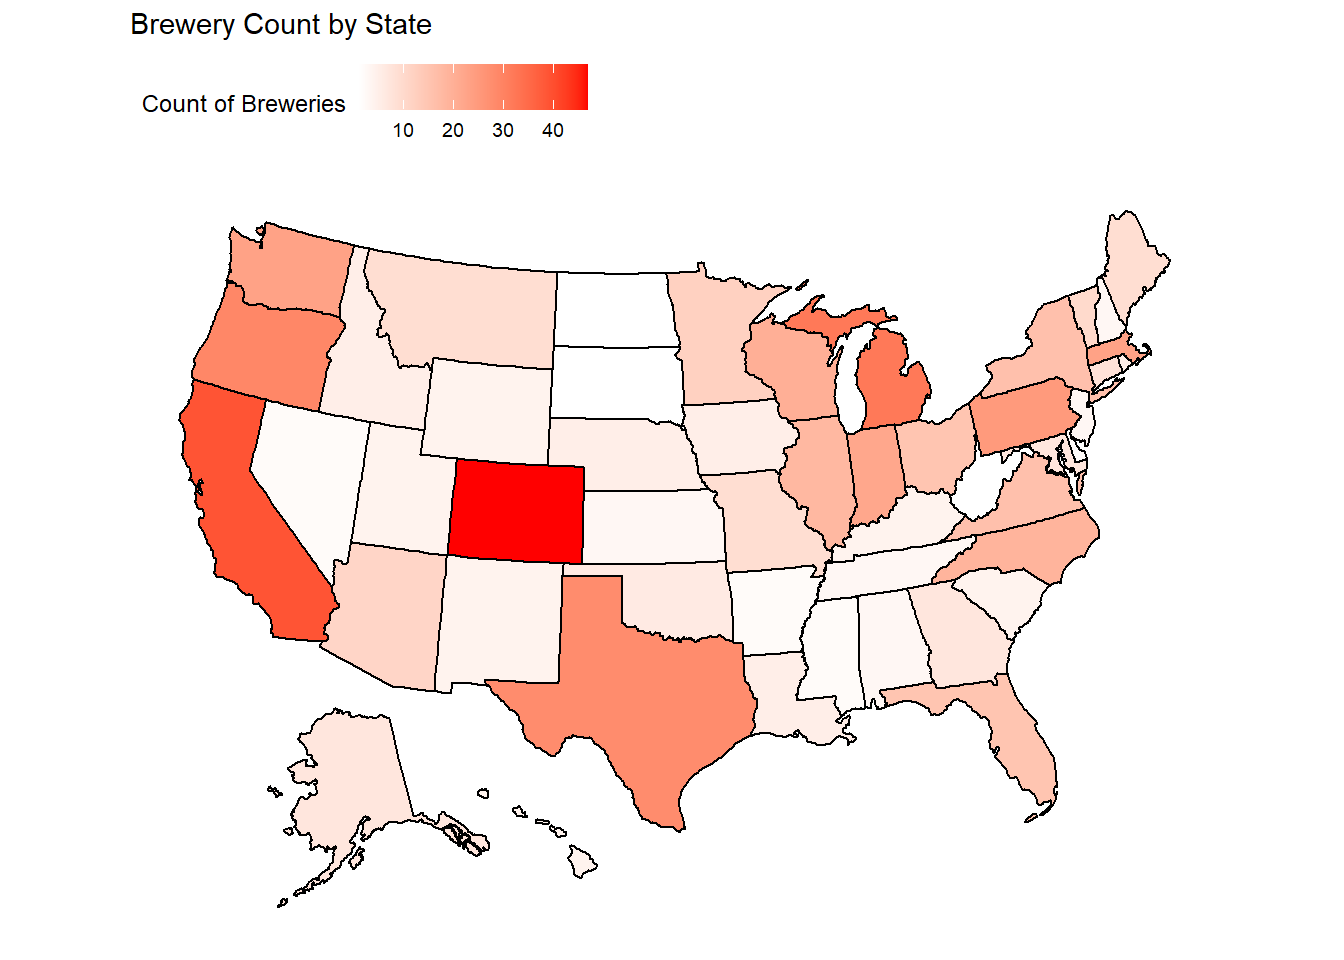
\includegraphics{CaseStudy2DDS_files/figure-latex/unnamed-chunk-2-1.pdf}

\begin{Shaded}
\begin{Highlighting}[]
\NormalTok{corr_data_n <-}\StringTok{ }\NormalTok{data }\OperatorTok\StringTok{ }\KeywordTok{filter}\NormalTok{(Attrition }\OperatorTok{==}\StringTok{"No"}\NormalTok{) }\OperatorTok\StringTok{ }\KeywordTok{select}\NormalTok{(Age, TotalWorkingYears, YearsAtCompany, YearsSinceLastPromotion, YearsInCurrentRole, YearsWithCurrManager, MonthlyIncome,TrainingTimesLastYear,StockOptionLevel,PercentSalaryHike,NumCompaniesWorked,DistanceFromHome)}

\NormalTok{corr <-}\StringTok{ }\KeywordTok{round}\NormalTok{(}\KeywordTok{cor}\NormalTok{(corr_data_n),}\DecValTok{1}\NormalTok{)}

\KeywordTok{ggcorrplot}\NormalTok{(corr, }\DataTypeTok{hc.order =} \OtherTok{TRUE}\NormalTok{, }
           \DataTypeTok{type =} \StringTok{"lower"}\NormalTok{, }
           \DataTypeTok{lab =} \OtherTok{TRUE}\NormalTok{, }
           \DataTypeTok{lab_size =} \DecValTok{3}\NormalTok{, }
           \DataTypeTok{method=}\StringTok{"circle"}\NormalTok{, }
           \DataTypeTok{colors =} \KeywordTok{c}\NormalTok{(}\StringTok{"red"}\NormalTok{, }\StringTok{"white"}\NormalTok{, }\StringTok{"springgreen3"}\NormalTok{), }
           \DataTypeTok{title=}\StringTok{"Continuous Variables without Attrition"}\NormalTok{, }
           \DataTypeTok{ggtheme=}\NormalTok{theme_bw)}
\end{Highlighting}
\end{Shaded}

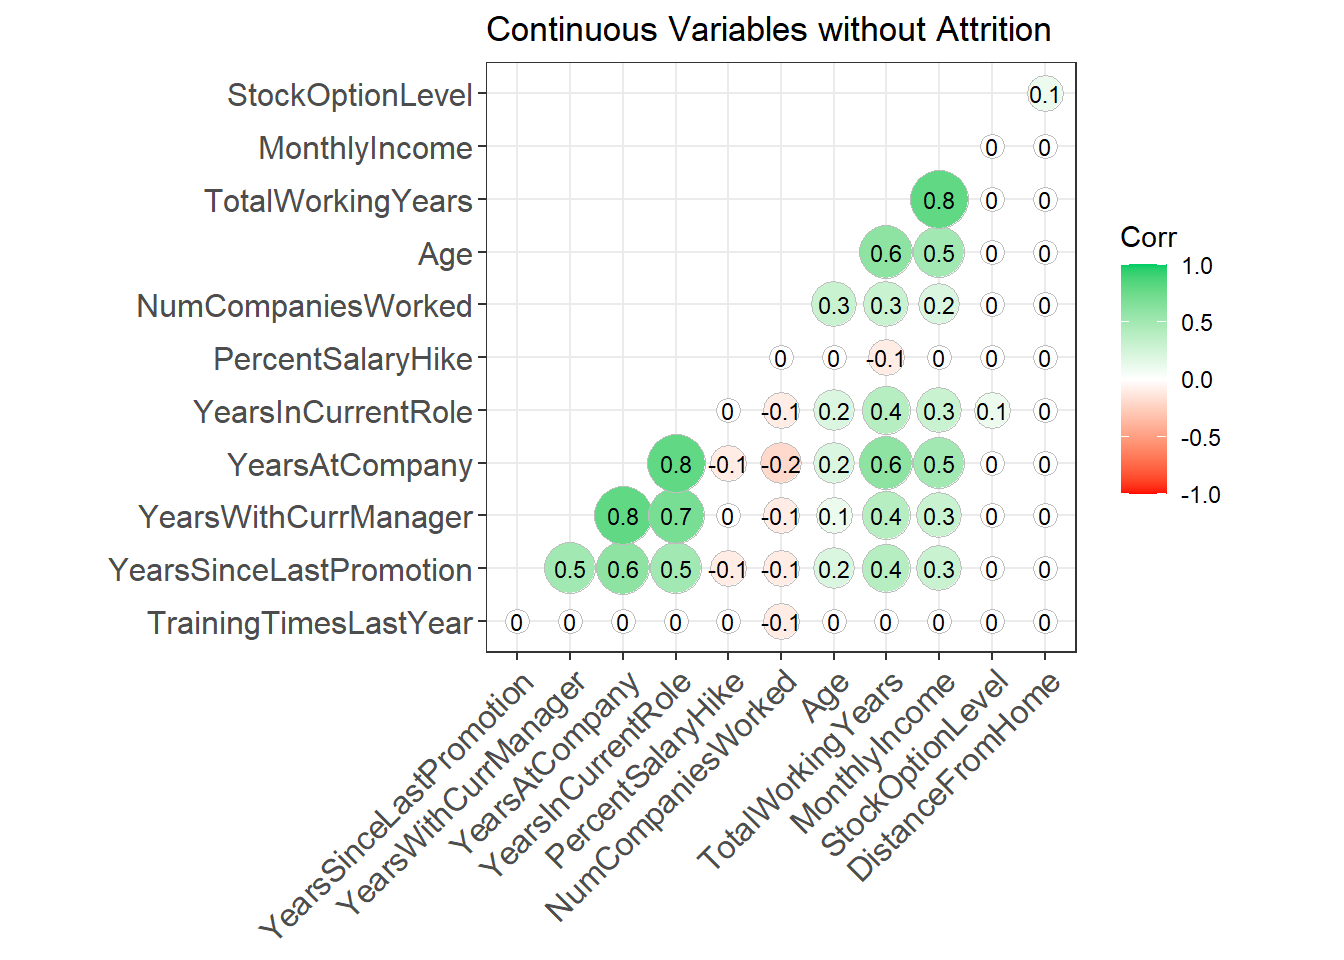
\includegraphics{CaseStudy2DDS_files/figure-latex/unnamed-chunk-2-2.pdf}
\#\# TTest - testing the 5 most significant varables

\begin{Shaded}
\begin{Highlighting}[]
\CommentTok{# we will be using a T test here because we would like to know: does this variable lead to a difference in attrition?}
\CommentTok{# if we have a samll P value that means this varable does show a difference in means betwwen attrition and not.}

\NormalTok{att_mi <-}\StringTok{ }\NormalTok{data }\OperatorTok\StringTok{ }\KeywordTok{filter}\NormalTok{(Attrition}\OperatorTok{==}\StringTok{"Yes"}\NormalTok{) }\OperatorTok\StringTok{ }\KeywordTok{select}\NormalTok{(MonthlyIncome)}
\NormalTok{stay_mi <-}\StringTok{ }\NormalTok{data }\OperatorTok\StringTok{ }\KeywordTok{filter}\NormalTok{(Attrition}\OperatorTok{==}\StringTok{"No"}\NormalTok{) }\OperatorTok\StringTok{ }\KeywordTok{select}\NormalTok{(MonthlyIncome)}
\NormalTok{mi_t <-}\KeywordTok{t.test}\NormalTok{(att_mi, stay_mi, }\DataTypeTok{alternative=}\StringTok{"two.sided"}\NormalTok{)}

\NormalTok{att_twy <-}\StringTok{ }\NormalTok{data }\OperatorTok\StringTok{ }\KeywordTok{filter}\NormalTok{(Attrition}\OperatorTok{==}\StringTok{"Yes"}\NormalTok{) }\OperatorTok\StringTok{ }\KeywordTok{select}\NormalTok{(TotalWorkingYears)}
\NormalTok{stay_twy <-}\StringTok{ }\NormalTok{data }\OperatorTok\StringTok{ }\KeywordTok{filter}\NormalTok{(Attrition}\OperatorTok{==}\StringTok{"No"}\NormalTok{) }\OperatorTok\StringTok{ }\KeywordTok{select}\NormalTok{(TotalWorkingYears)}
\NormalTok{twy_t <-}\KeywordTok{t.test}\NormalTok{(att_twy, stay_twy, }\DataTypeTok{alternative=}\StringTok{"two.sided"}\NormalTok{)}

\NormalTok{att_yicr <-}\StringTok{ }\NormalTok{data }\OperatorTok\StringTok{ }\KeywordTok{filter}\NormalTok{(Attrition}\OperatorTok{==}\StringTok{"Yes"}\NormalTok{) }\OperatorTok\StringTok{ }\KeywordTok{select}\NormalTok{(YearsInCurrentRole)}
\NormalTok{stay_yicr <-}\StringTok{ }\NormalTok{data }\OperatorTok\StringTok{ }\KeywordTok{filter}\NormalTok{(Attrition}\OperatorTok{==}\StringTok{"No"}\NormalTok{) }\OperatorTok\StringTok{ }\KeywordTok{select}\NormalTok{(YearsInCurrentRole)}
\NormalTok{yicr <-}\StringTok{ }\KeywordTok{t.test}\NormalTok{(att_yicr, stay_yicr, }\DataTypeTok{alternative=}\StringTok{"two.sided"}\NormalTok{)}

\NormalTok{att_ywcm <-}\StringTok{ }\NormalTok{data }\OperatorTok\StringTok{ }\KeywordTok{filter}\NormalTok{(Attrition}\OperatorTok{==}\StringTok{"Yes"}\NormalTok{) }\OperatorTok\StringTok{ }\KeywordTok{select}\NormalTok{(YearsWithCurrManager)}
\NormalTok{stay_ywcm <-}\StringTok{ }\NormalTok{data }\OperatorTok\StringTok{ }\KeywordTok{filter}\NormalTok{(Attrition}\OperatorTok{==}\StringTok{"No"}\NormalTok{) }\OperatorTok\StringTok{ }\KeywordTok{select}\NormalTok{(YearsWithCurrManager)}
\NormalTok{ywcm <-}\StringTok{ }\KeywordTok{t.test}\NormalTok{(att_ywcm, stay_ywcm, }\DataTypeTok{alternative=}\StringTok{"two.sided"}\NormalTok{)}

\NormalTok{att_yac <-}\StringTok{ }\NormalTok{data }\OperatorTok\StringTok{ }\KeywordTok{filter}\NormalTok{(Attrition}\OperatorTok{==}\StringTok{"Yes"}\NormalTok{) }\OperatorTok\StringTok{ }\KeywordTok{select}\NormalTok{(YearsAtCompany)}
\NormalTok{stay_yac <-}\StringTok{ }\NormalTok{data }\OperatorTok\StringTok{ }\KeywordTok{filter}\NormalTok{(Attrition}\OperatorTok{==}\StringTok{"No"}\NormalTok{) }\OperatorTok\StringTok{ }\KeywordTok{select}\NormalTok{(YearsAtCompany)}
\NormalTok{yac <-}\StringTok{ }\KeywordTok{t.test}\NormalTok{(att_yac, stay_yac, }\DataTypeTok{alternative=}\StringTok{"two.sided"}\NormalTok{)}

\NormalTok{cont_var =}\StringTok{ }\KeywordTok{c}\NormalTok{(}\StringTok{"MonthlyIncome"}\NormalTok{, }\StringTok{"TotalWorkingYears"}\NormalTok{,}\StringTok{"YearsInCurrentRole"}\NormalTok{,}\StringTok{"YearsWithCurrManager"}\NormalTok{,}\StringTok{"YearsAtCompany"}\NormalTok{)}
\NormalTok{ttest_p =}\StringTok{ }\KeywordTok{c}\NormalTok{(mi_t}\OperatorTok{$}\NormalTok{p.value, twy_t}\OperatorTok{$}\NormalTok{p.value, yicr}\OperatorTok{$}\NormalTok{p.value, ywcm}\OperatorTok{$}\NormalTok{p.value, yac}\OperatorTok{$}\NormalTok{p.value)}

\NormalTok{df1_ttest =}\StringTok{ }\KeywordTok{data.frame}\NormalTok{(}\DataTypeTok{Variable=}\NormalTok{cont_var, }\StringTok{"T-Test pvalue"}\NormalTok{=ttest_p)}
\KeywordTok{gt}\NormalTok{(df1_ttest)}
\end{Highlighting}
\end{Shaded}

\captionsetup[table]{labelformat=empty,skip=1pt}
\begin{longtable}{lr}
\toprule
Variable & T.Test.pvalue \\ 
\midrule
MonthlyIncome & 2.412488e-07 \\ 
TotalWorkingYears & 6.595682e-07 \\ 
YearsInCurrentRole & 1.522152e-06 \\ 
YearsWithCurrManager & 5.084229e-06 \\ 
YearsAtCompany & 2.563021e-04 \\ 
\bottomrule
\end{longtable}

\begin{Shaded}
\begin{Highlighting}[]
\NormalTok{df1_ttest}
\end{Highlighting}
\end{Shaded}

\begin{verbatim}
##               Variable T.Test.pvalue
## 1        MonthlyIncome  2.412488e-07
## 2    TotalWorkingYears  6.595682e-07
## 3   YearsInCurrentRole  1.522152e-06
## 4 YearsWithCurrManager  5.084229e-06
## 5       YearsAtCompany  2.563021e-04
\end{verbatim}

\hypertarget{showing-off-the-most-significant-continious-varables.}{%
\subsection{showing off the most significant continious
varables.}\label{showing-off-the-most-significant-continious-varables.}}

\begin{Shaded}
\begin{Highlighting}[]
\CommentTok{#these varables appear to be significant}
\NormalTok{mi_plot <-data }\OperatorTok\StringTok{ }\KeywordTok{ggplot}\NormalTok{(}\KeywordTok{aes}\NormalTok{(MonthlyIncome))}\OperatorTok{+}
\StringTok{  }\KeywordTok{geom_density}\NormalTok{(}\KeywordTok{aes}\NormalTok{(}\DataTypeTok{fill=}\NormalTok{Attrition))}\OperatorTok{+}
\StringTok{  }\KeywordTok{labs}\NormalTok{(}\DataTypeTok{title=}\StringTok{"Monthly Income vs Attrition"}\NormalTok{)}\OperatorTok{+}
\StringTok{  }\KeywordTok{xlab}\NormalTok{(}\StringTok{"Monthly Income"}\NormalTok{)}

\NormalTok{twy_plot <-data }\OperatorTok\StringTok{ }\KeywordTok{ggplot}\NormalTok{(}\KeywordTok{aes}\NormalTok{(TotalWorkingYears))}\OperatorTok{+}
\StringTok{  }\KeywordTok{geom_density}\NormalTok{(}\KeywordTok{aes}\NormalTok{(}\DataTypeTok{fill=}\NormalTok{Attrition))}\OperatorTok{+}
\StringTok{  }\KeywordTok{labs}\NormalTok{(}\DataTypeTok{title=}\StringTok{"Total Working Years vs Attrition"}\NormalTok{)}\OperatorTok{+}
\StringTok{  }\KeywordTok{xlab}\NormalTok{(}\StringTok{"Total Working Years"}\NormalTok{)}

\NormalTok{yac_plot <-}\StringTok{ }\NormalTok{data }\OperatorTok\StringTok{ }\KeywordTok{ggplot}\NormalTok{(}\KeywordTok{aes}\NormalTok{(YearsAtCompany))}\OperatorTok{+}
\StringTok{  }\KeywordTok{geom_density}\NormalTok{(}\KeywordTok{aes}\NormalTok{(}\DataTypeTok{fill=}\NormalTok{Attrition))}\OperatorTok{+}
\StringTok{  }\KeywordTok{labs}\NormalTok{(}\DataTypeTok{title=}\StringTok{"Years At the Company vs Attrition"}\NormalTok{)}\OperatorTok{+}
\StringTok{  }\KeywordTok{xlab}\NormalTok{(}\StringTok{"Years at the Company"}\NormalTok{)}

\NormalTok{yicr_plot <-}\StringTok{ }\NormalTok{data }\OperatorTok\StringTok{ }\KeywordTok{ggplot}\NormalTok{(}\KeywordTok{aes}\NormalTok{(YearsInCurrentRole))}\OperatorTok{+}
\StringTok{  }\KeywordTok{geom_density}\NormalTok{(}\KeywordTok{aes}\NormalTok{(}\DataTypeTok{fill=}\NormalTok{Attrition))}\OperatorTok{+}
\StringTok{  }\KeywordTok{labs}\NormalTok{(}\DataTypeTok{title=}\StringTok{"Years In Current Role vs Attrition"}\NormalTok{)}\OperatorTok{+}
\StringTok{  }\KeywordTok{xlab}\NormalTok{(}\StringTok{"Years in Current Role"}\NormalTok{)}

\NormalTok{ywcm_plot <-}\StringTok{ }\NormalTok{data }\OperatorTok\StringTok{ }\KeywordTok{ggplot}\NormalTok{(}\KeywordTok{aes}\NormalTok{(YearsWithCurrManager))}\OperatorTok{+}
\StringTok{  }\KeywordTok{geom_density}\NormalTok{(}\KeywordTok{aes}\NormalTok{(}\DataTypeTok{fill=}\NormalTok{Attrition))}\OperatorTok{+}
\StringTok{  }\KeywordTok{labs}\NormalTok{(}\DataTypeTok{title=}\StringTok{"Years With Current Manager vs Attrition"}\NormalTok{)}\OperatorTok{+}
\StringTok{  }\KeywordTok{xlab}\NormalTok{(}\StringTok{"Years with Current Manager"}\NormalTok{)}

\KeywordTok{grid.arrange}\NormalTok{(mi_plot,twy_plot,yac_plot,yicr_plot,ywcm_plot)}
\end{Highlighting}
\end{Shaded}

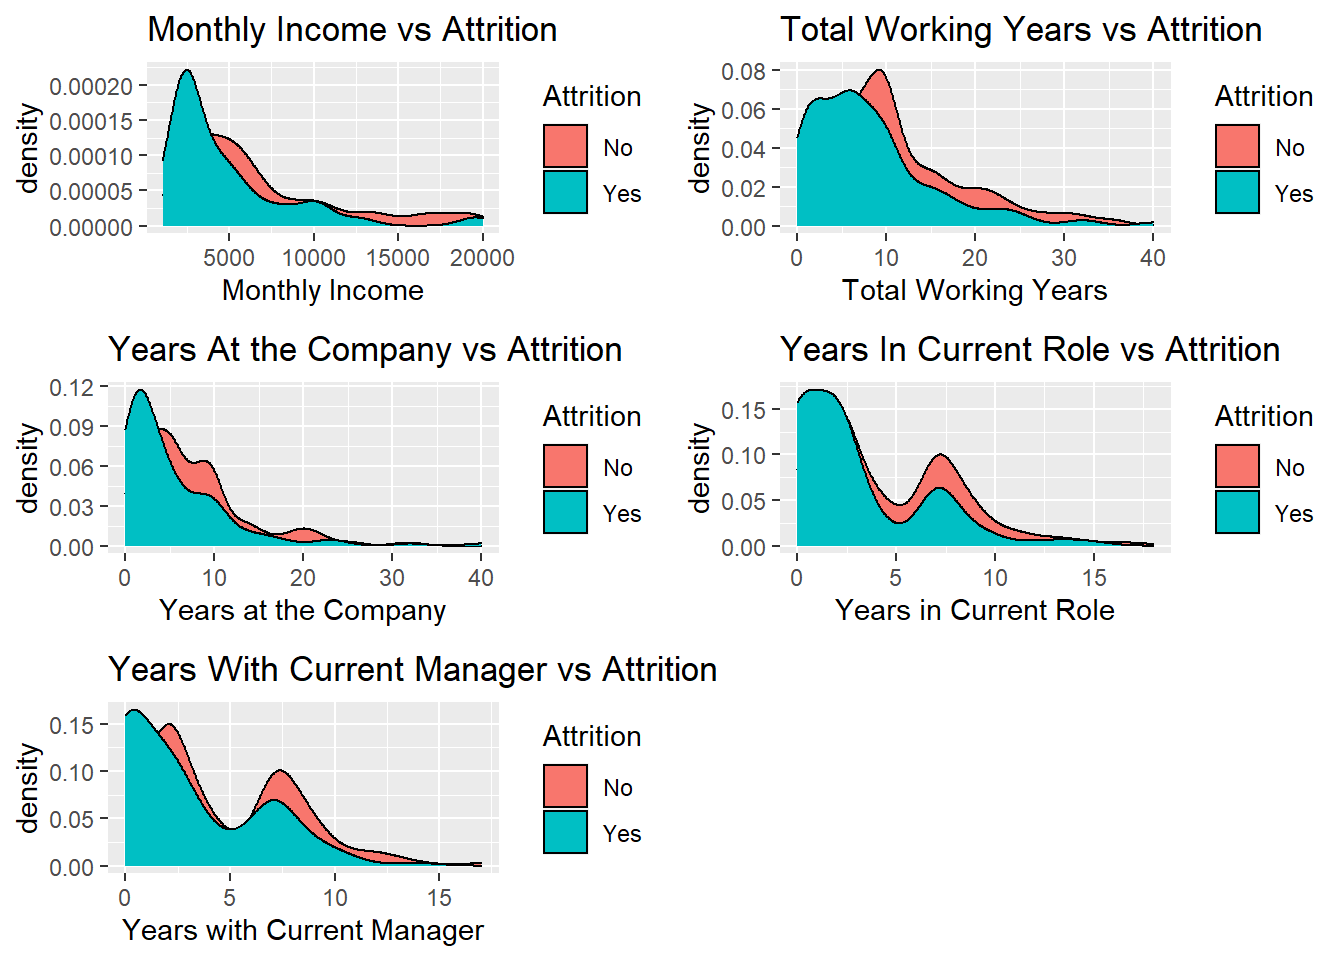
\includegraphics{CaseStudy2DDS_files/figure-latex/unnamed-chunk-4-1.pdf}

\begin{Shaded}
\begin{Highlighting}[]
\CommentTok{# show both density and box charts}
\end{Highlighting}
\end{Shaded}

\begin{Shaded}
\begin{Highlighting}[]
\CommentTok{# show the same data as above but in boxplot}
\NormalTok{mi_plot_box <-data }\OperatorTok\StringTok{ }\KeywordTok{ggplot}\NormalTok{(}\KeywordTok{aes}\NormalTok{(MonthlyIncome))}\OperatorTok{+}
\StringTok{  }\KeywordTok{geom_boxplot}\NormalTok{(}\KeywordTok{aes}\NormalTok{(}\DataTypeTok{fill=}\NormalTok{Attrition))}\OperatorTok{+}
\StringTok{  }\KeywordTok{labs}\NormalTok{(}\DataTypeTok{title=}\StringTok{"Monthly Income vs Attrition"}\NormalTok{)}\OperatorTok{+}
\StringTok{  }\KeywordTok{xlab}\NormalTok{(}\StringTok{"Monthly Income"}\NormalTok{)}

\NormalTok{twy_plot_box <-data }\OperatorTok\StringTok{ }\KeywordTok{ggplot}\NormalTok{(}\KeywordTok{aes}\NormalTok{(TotalWorkingYears))}\OperatorTok{+}
\StringTok{  }\KeywordTok{geom_boxplot}\NormalTok{(}\KeywordTok{aes}\NormalTok{(}\DataTypeTok{fill=}\NormalTok{Attrition))}\OperatorTok{+}
\StringTok{  }\KeywordTok{labs}\NormalTok{(}\DataTypeTok{title=}\StringTok{"Total Working Years vs Attrition"}\NormalTok{)}\OperatorTok{+}
\StringTok{  }\KeywordTok{xlab}\NormalTok{(}\StringTok{"Total Working Years"}\NormalTok{)}

\NormalTok{yac_plot_box <-}\StringTok{ }\NormalTok{data }\OperatorTok\StringTok{ }\KeywordTok{ggplot}\NormalTok{(}\KeywordTok{aes}\NormalTok{(YearsAtCompany))}\OperatorTok{+}
\StringTok{  }\KeywordTok{geom_boxplot}\NormalTok{(}\KeywordTok{aes}\NormalTok{(}\DataTypeTok{fill=}\NormalTok{Attrition))}\OperatorTok{+}
\StringTok{  }\KeywordTok{labs}\NormalTok{(}\DataTypeTok{title=}\StringTok{"Years At the Company vs Attrition"}\NormalTok{)}\OperatorTok{+}
\StringTok{  }\KeywordTok{xlab}\NormalTok{(}\StringTok{"Years at the COmpany"}\NormalTok{)}

\NormalTok{yicr_plot_box <-}\StringTok{ }\NormalTok{data }\OperatorTok\StringTok{ }\KeywordTok{ggplot}\NormalTok{(}\KeywordTok{aes}\NormalTok{(YearsInCurrentRole))}\OperatorTok{+}
\StringTok{  }\KeywordTok{geom_boxplot}\NormalTok{(}\KeywordTok{aes}\NormalTok{(}\DataTypeTok{fill=}\NormalTok{Attrition))}\OperatorTok{+}
\StringTok{  }\KeywordTok{labs}\NormalTok{(}\DataTypeTok{title=}\StringTok{"Years In Current Role vs Attrition"}\NormalTok{)}\OperatorTok{+}
\StringTok{  }\KeywordTok{xlab}\NormalTok{(}\StringTok{"Years in Current Role"}\NormalTok{)}

\NormalTok{ywcm_plot_box <-}\StringTok{ }\NormalTok{data }\OperatorTok\StringTok{ }\KeywordTok{ggplot}\NormalTok{(}\KeywordTok{aes}\NormalTok{(YearsWithCurrManager))}\OperatorTok{+}
\StringTok{  }\KeywordTok{geom_boxplot}\NormalTok{(}\KeywordTok{aes}\NormalTok{(}\DataTypeTok{fill=}\NormalTok{Attrition))}\OperatorTok{+}
\StringTok{  }\KeywordTok{labs}\NormalTok{(}\DataTypeTok{title=}\StringTok{"Years With Current Manager vs Attrition"}\NormalTok{)}\OperatorTok{+}
\StringTok{  }\KeywordTok{xlab}\NormalTok{(}\StringTok{"Years with Current Manager"}\NormalTok{)}

\KeywordTok{grid.arrange}\NormalTok{(mi_plot_box,twy_plot_box,yac_plot_box,yicr_plot_box,ywcm_plot_box)}
\end{Highlighting}
\end{Shaded}

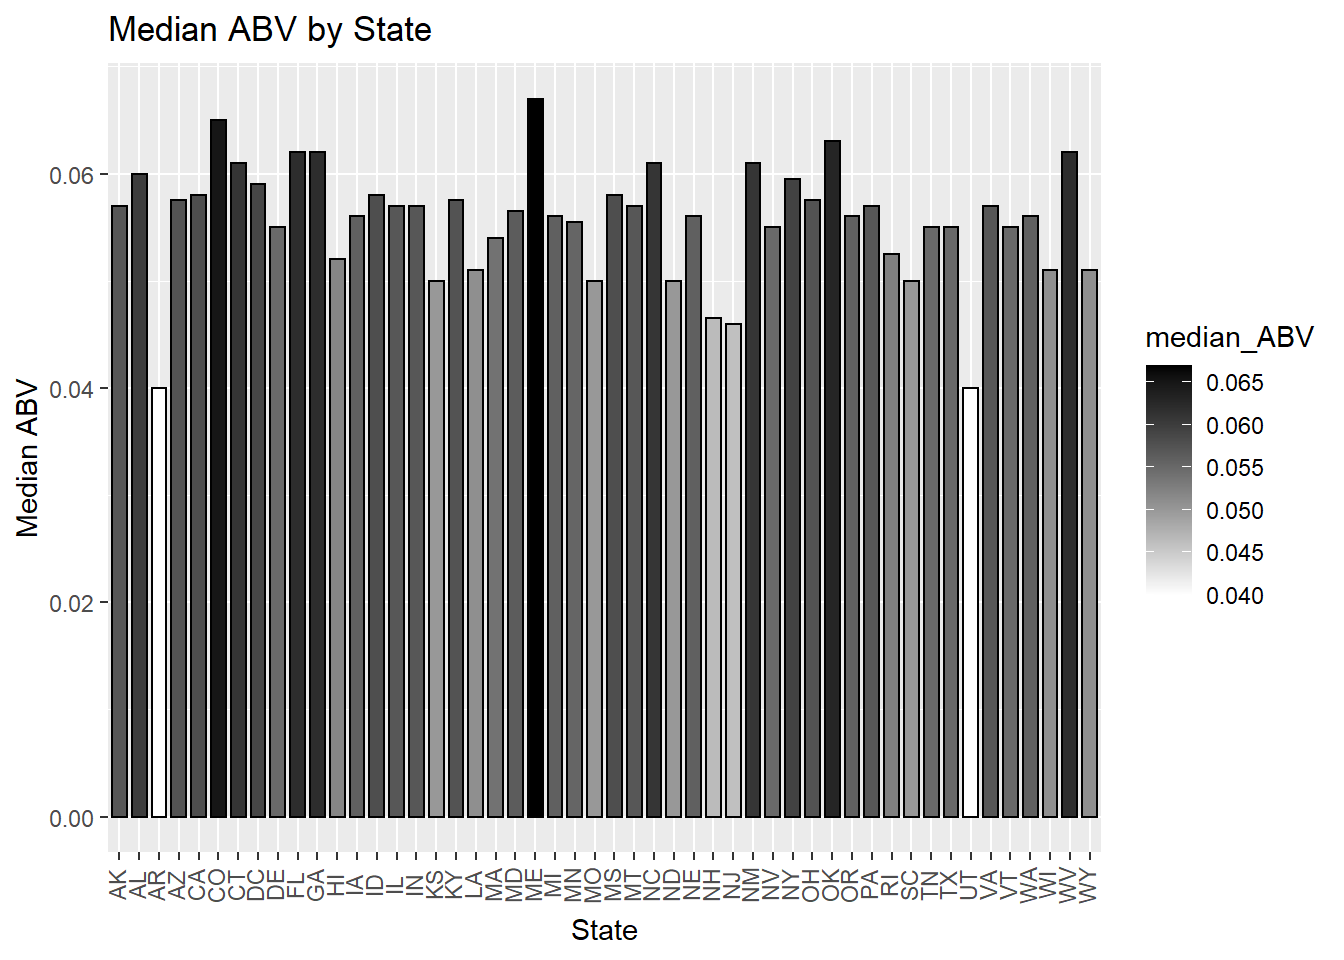
\includegraphics{CaseStudy2DDS_files/figure-latex/unnamed-chunk-5-1.pdf}

\hypertarget{wrangling-categorical-varables}{%
\subsection{wrangling categorical
varables}\label{wrangling-categorical-varables}}

\hypertarget{calculating-the-proportion}{%
\subsection{calculating the
proportion}\label{calculating-the-proportion}}

\hypertarget{varables-with-little-relationship}{%
\subsection{varables with little
relationship}\label{varables-with-little-relationship}}

\begin{Shaded}
\begin{Highlighting}[]
\CommentTok{#data %>% group_by(PerformanceRating) %>% count(Attrition) %>% mutate(sum=sum(n)) %>% mutate(proportion=n/sum*100) %>% filter(Attrition=="Yes")}
\CommentTok{#data %>% group_by(RelationshipSatisfaction) %>% count(Attrition) %>% mutate(sum=sum(n)) %>% mutate(proportion=n/sum*100) %>% filter(Attrition=="Yes")}
\CommentTok{#data %>% group_by(Education) %>% count(Attrition) %>% mutate(sum=sum(n)) %>% mutate(proportion=n/sum*100) %>% filter(Attrition=="Yes")}
\CommentTok{#data %>% group_by(EducationField) %>% count(Attrition) %>% mutate(sum=sum(n)) %>% mutate(proportion=n/sum*100) %>% filter(Attrition=="Yes")}
\CommentTok{#data %>% group_by(Gender) %>% count(Attrition) %>% mutate(sum=sum(n)) %>% mutate(proportion=n/sum*100) %>% filter(Attrition=="Yes")}
\CommentTok{#data %>% group_by(BusinessTravel) %>% count(Attrition) %>% mutate(sum=sum(n)) %>% mutate(proportion=n/sum*100) %>% filter(Attrition=="Yes")}
\CommentTok{#data %>% group_by(Department) %>% count(Attrition) %>% mutate(sum=sum(n)) %>% mutate(proportion=n/sum*100) %>% filter(Attrition=="Yes")}
\CommentTok{#data %>% group_by(WorkLifeBalance) %>% count(Attrition) %>% mutate(sum=sum(n)) %>% mutate(proportion=n/sum*100) %>% filter(Attrition=="Yes")}
\CommentTok{#data %>% group_by(JobSatisfaction) %>% count(Attrition) %>% mutate(sum=sum(n)) %>% mutate(proportion=n/sum*100) %>% filter(Attrition=="Yes")}
\end{Highlighting}
\end{Shaded}

\hypertarget{categorical-varables-that-show-a-relatinship}{%
\subsection{Categorical varables that show a
relatinship}\label{categorical-varables-that-show-a-relatinship}}

\begin{Shaded}
\begin{Highlighting}[]
\NormalTok{data }\OperatorTok\StringTok{ }\KeywordTok{group_by}\NormalTok{(JobLevel) }\OperatorTok\StringTok{ }
\StringTok{  }\KeywordTok{count}\NormalTok{(Attrition) }\OperatorTok\StringTok{ }
\StringTok{  }\KeywordTok{mutate}\NormalTok{(}\DataTypeTok{sum=}\KeywordTok{sum}\NormalTok{(n)) }\OperatorTok\StringTok{ }
\StringTok{  }\KeywordTok{mutate}\NormalTok{(}\DataTypeTok{proportion=}\NormalTok{n}\OperatorTok{/}\NormalTok{sum}\OperatorTok{*}\DecValTok{100}\NormalTok{) }\OperatorTok\StringTok{ }
\StringTok{  }\KeywordTok{filter}\NormalTok{(Attrition}\OperatorTok{==}\StringTok{"Yes"}\NormalTok{)}
\end{Highlighting}
\end{Shaded}

\begin{verbatim}
## # A tibble: 5 x 5
## # Groups:   JobLevel [5]
##   JobLevel Attrition     n   sum proportion
##   <fct>    <chr>     <int> <int>      <dbl>
## 1 1        Yes          86   329      26.1 
## 2 2        Yes          30   312       9.62
## 3 3        Yes          17   132      12.9 
## 4 4        Yes           3    60       5   
## 5 5        Yes           4    37      10.8
\end{verbatim}

\begin{Shaded}
\begin{Highlighting}[]
\NormalTok{data }\OperatorTok\StringTok{ }\KeywordTok{group_by}\NormalTok{(OverTime) }\OperatorTok\StringTok{ }
\StringTok{  }\KeywordTok{count}\NormalTok{(Attrition) }\OperatorTok\StringTok{ }
\StringTok{  }\KeywordTok{mutate}\NormalTok{(}\DataTypeTok{sum=}\KeywordTok{sum}\NormalTok{(n)) }\OperatorTok\StringTok{ }
\StringTok{  }\KeywordTok{mutate}\NormalTok{(}\DataTypeTok{proportion=}\NormalTok{n}\OperatorTok{/}\NormalTok{sum}\OperatorTok{*}\DecValTok{100}\NormalTok{) }\OperatorTok\StringTok{ }
\StringTok{  }\KeywordTok{filter}\NormalTok{(Attrition}\OperatorTok{==}\StringTok{"Yes"}\NormalTok{)}
\end{Highlighting}
\end{Shaded}

\begin{verbatim}
## # A tibble: 2 x 5
## # Groups:   OverTime [2]
##   OverTime Attrition     n   sum proportion
##   <chr>    <chr>     <int> <int>      <dbl>
## 1 No       Yes          60   618       9.71
## 2 Yes      Yes          80   252      31.7
\end{verbatim}

\begin{Shaded}
\begin{Highlighting}[]
\NormalTok{data }\OperatorTok\StringTok{ }\KeywordTok{group_by}\NormalTok{(JobInvolvement) }\OperatorTok\StringTok{ }
\StringTok{  }\KeywordTok{count}\NormalTok{(Attrition) }\OperatorTok\StringTok{ }
\StringTok{  }\KeywordTok{mutate}\NormalTok{(}\DataTypeTok{sum=}\KeywordTok{sum}\NormalTok{(n)) }\OperatorTok\StringTok{ }
\StringTok{  }\KeywordTok{mutate}\NormalTok{(}\DataTypeTok{proportion=}\NormalTok{n}\OperatorTok{/}\NormalTok{sum}\OperatorTok{*}\DecValTok{100}\NormalTok{) }\OperatorTok\StringTok{ }
\StringTok{  }\KeywordTok{filter}\NormalTok{(Attrition}\OperatorTok{==}\StringTok{"Yes"}\NormalTok{)}
\end{Highlighting}
\end{Shaded}

\begin{verbatim}
## # A tibble: 4 x 5
## # Groups:   JobInvolvement [4]
##   JobInvolvement Attrition     n   sum proportion
##   <fct>          <chr>     <int> <int>      <dbl>
## 1 1              Yes          22    47      46.8 
## 2 2              Yes          44   228      19.3 
## 3 3              Yes          67   514      13.0 
## 4 4              Yes           7    81       8.64
\end{verbatim}

\begin{Shaded}
\begin{Highlighting}[]
\NormalTok{data }\OperatorTok\StringTok{ }\KeywordTok{group_by}\NormalTok{(JobRole) }\OperatorTok\StringTok{ }
\StringTok{  }\KeywordTok{count}\NormalTok{(Attrition) }\OperatorTok\StringTok{ }
\StringTok{  }\KeywordTok{mutate}\NormalTok{(}\DataTypeTok{sum=}\KeywordTok{sum}\NormalTok{(n)) }\OperatorTok\StringTok{ }
\StringTok{  }\KeywordTok{mutate}\NormalTok{(}\DataTypeTok{proportion=}\NormalTok{n}\OperatorTok{/}\NormalTok{sum}\OperatorTok{*}\DecValTok{100}\NormalTok{) }\OperatorTok\StringTok{ }
\StringTok{  }\KeywordTok{filter}\NormalTok{(Attrition}\OperatorTok{==}\StringTok{"Yes"}\NormalTok{)}
\end{Highlighting}
\end{Shaded}

\begin{verbatim}
## # A tibble: 9 x 5
## # Groups:   JobRole [9]
##   JobRole                   Attrition     n   sum proportion
##   <chr>                     <chr>     <int> <int>      <dbl>
## 1 Healthcare Representative Yes           8    76      10.5 
## 2 Human Resources           Yes           6    27      22.2 
## 3 Laboratory Technician     Yes          30   153      19.6 
## 4 Manager                   Yes           4    51       7.84
## 5 Manufacturing Director    Yes           2    87       2.30
## 6 Research Director         Yes           1    51       1.96
## 7 Research Scientist        Yes          32   172      18.6 
## 8 Sales Executive           Yes          33   200      16.5 
## 9 Sales Representative      Yes          24    53      45.3
\end{verbatim}

\begin{Shaded}
\begin{Highlighting}[]
\NormalTok{data }\OperatorTok\StringTok{ }\KeywordTok{group_by}\NormalTok{(MaritalStatus) }\OperatorTok\StringTok{ }
\StringTok{  }\KeywordTok{count}\NormalTok{(Attrition) }\OperatorTok\StringTok{ }
\StringTok{  }\KeywordTok{mutate}\NormalTok{(}\DataTypeTok{sum=}\KeywordTok{sum}\NormalTok{(n)) }\OperatorTok\StringTok{ }
\StringTok{  }\KeywordTok{mutate}\NormalTok{(}\DataTypeTok{proportion=}\NormalTok{n}\OperatorTok{/}\NormalTok{sum}\OperatorTok{*}\DecValTok{100}\NormalTok{) }\OperatorTok\StringTok{ }
\StringTok{  }\KeywordTok{filter}\NormalTok{(Attrition}\OperatorTok{==}\StringTok{"Yes"}\NormalTok{)}
\end{Highlighting}
\end{Shaded}

\begin{verbatim}
## # A tibble: 3 x 5
## # Groups:   MaritalStatus [3]
##   MaritalStatus Attrition     n   sum proportion
##   <chr>         <chr>     <int> <int>      <dbl>
## 1 Divorced      Yes          12   191       6.28
## 2 Married       Yes          58   410      14.1 
## 3 Single        Yes          70   269      26.0
\end{verbatim}

\hypertarget{plotting-the-categorical-varables}{%
\subsection{Plotting the Categorical
varables}\label{plotting-the-categorical-varables}}

\begin{Shaded}
\begin{Highlighting}[]
\KeywordTok{library}\NormalTok{(patchwork)}
\end{Highlighting}
\end{Shaded}

\begin{verbatim}
## Warning: package 'patchwork' was built under R version 4.0.5
\end{verbatim}

\begin{Shaded}
\begin{Highlighting}[]
\NormalTok{JL_chi <-}\StringTok{ }\KeywordTok{chisq.test}\NormalTok{(data}\OperatorTok{$}\NormalTok{JobLevel, data}\OperatorTok{$}\NormalTok{Attrition)}
\NormalTok{O_chi <-}\StringTok{ }\KeywordTok{chisq.test}\NormalTok{(data}\OperatorTok{$}\NormalTok{OverTime, data}\OperatorTok{$}\NormalTok{Attrition)}
\NormalTok{JI_chi <-}\StringTok{ }\KeywordTok{chisq.test}\NormalTok{(data}\OperatorTok{$}\NormalTok{JobInvolvement, data}\OperatorTok{$}\NormalTok{Attrition)}
\NormalTok{JR_chi <-}\StringTok{ }\KeywordTok{chisq.test}\NormalTok{(data}\OperatorTok{$}\NormalTok{JobRole, data}\OperatorTok{$}\NormalTok{Attrition)}
\end{Highlighting}
\end{Shaded}

\begin{verbatim}
## Warning in chisq.test(data$JobRole, data$Attrition): Chi-squared approximation may be incorrect
\end{verbatim}

\begin{Shaded}
\begin{Highlighting}[]
\NormalTok{MS_chi <-}\StringTok{ }\KeywordTok{chisq.test}\NormalTok{(data}\OperatorTok{$}\NormalTok{MaritalStatus, data}\OperatorTok{$}\NormalTok{Attrition)}

\NormalTok{cat_var =}\StringTok{ }\KeywordTok{c}\NormalTok{(}\StringTok{"JobLevel"}\NormalTok{, }\StringTok{"OverTime"}\NormalTok{, }\StringTok{"JobInvolvement"}\NormalTok{, }\StringTok{"JobRole"}\NormalTok{, }\StringTok{"MaritalStatus"}\NormalTok{)}
\NormalTok{chi_p =}\StringTok{ }\KeywordTok{c}\NormalTok{(JL_chi}\OperatorTok{$}\NormalTok{p.value, O_chi}\OperatorTok{$}\NormalTok{p.value, JI_chi}\OperatorTok{$}\NormalTok{p.value, JR_chi}\OperatorTok{$}\NormalTok{p.value, MS_chi}\OperatorTok{$}\NormalTok{p.value)}
\NormalTok{df_chitest =}\StringTok{ }\KeywordTok{data.frame}\NormalTok{(}\DataTypeTok{Variable=}\NormalTok{cat_var, }\DataTypeTok{Chisq.pvalue=}\NormalTok{chi_p)}

\NormalTok{JL_plot <-}\StringTok{ }\NormalTok{data }\OperatorTok\StringTok{ }\KeywordTok{ggplot}\NormalTok{(}\KeywordTok{aes}\NormalTok{(JobLevel))}\OperatorTok{+}\KeywordTok{geom_bar}\NormalTok{(}\KeywordTok{aes}\NormalTok{(}\DataTypeTok{fill=}\NormalTok{Attrition)) }\OperatorTok{+}\StringTok{ }\KeywordTok{labs}\NormalTok{(}\DataTypeTok{title=}\StringTok{"JobLevel vs Attrition"}\NormalTok{)}\OperatorTok{+}\KeywordTok{coord_flip}\NormalTok{()}
\NormalTok{O_plot <-}\StringTok{ }\NormalTok{data }\OperatorTok\StringTok{ }\KeywordTok{ggplot}\NormalTok{(}\KeywordTok{aes}\NormalTok{(OverTime))}\OperatorTok{+}\KeywordTok{geom_bar}\NormalTok{(}\KeywordTok{aes}\NormalTok{(}\DataTypeTok{fill=}\NormalTok{Attrition)) }\OperatorTok{+}\StringTok{ }\KeywordTok{labs}\NormalTok{(}\DataTypeTok{title=}\StringTok{"Overtime vs Attrition"}\NormalTok{)}\OperatorTok{+}\KeywordTok{coord_flip}\NormalTok{()}
\NormalTok{JI_plot <-}\StringTok{ }\NormalTok{data }\OperatorTok\StringTok{ }\KeywordTok{ggplot}\NormalTok{(}\KeywordTok{aes}\NormalTok{(JobInvolvement))}\OperatorTok{+}\KeywordTok{geom_bar}\NormalTok{(}\KeywordTok{aes}\NormalTok{(}\DataTypeTok{fill=}\NormalTok{Attrition)) }\OperatorTok{+}\StringTok{ }\KeywordTok{labs}\NormalTok{(}\DataTypeTok{title=}\StringTok{"JobInvolvement vs Attrition"}\NormalTok{)}\OperatorTok{+}\KeywordTok{coord_flip}\NormalTok{()}
\NormalTok{JS_plot <-}\StringTok{ }\NormalTok{data }\OperatorTok\StringTok{ }\KeywordTok{ggplot}\NormalTok{(}\KeywordTok{aes}\NormalTok{(JobSatisfaction))}\OperatorTok{+}\KeywordTok{geom_bar}\NormalTok{(}\KeywordTok{aes}\NormalTok{(}\DataTypeTok{fill=}\NormalTok{Attrition)) }\OperatorTok{+}\StringTok{ }\KeywordTok{labs}\NormalTok{(}\DataTypeTok{title=}\StringTok{"JobSatisfaction vs Attrition"}\NormalTok{)}\OperatorTok{+}\KeywordTok{coord_flip}\NormalTok{()}
\NormalTok{JR_plot <-data }\OperatorTok\StringTok{ }\KeywordTok{ggplot}\NormalTok{(}\KeywordTok{aes}\NormalTok{(JobRole))}\OperatorTok{+}\KeywordTok{geom_bar}\NormalTok{(}\KeywordTok{aes}\NormalTok{(}\DataTypeTok{fill=}\NormalTok{Attrition)) }\OperatorTok{+}\StringTok{ }\KeywordTok{labs}\NormalTok{(}\DataTypeTok{title=}\StringTok{"JobRole vs Attrition"}\NormalTok{)}\OperatorTok{+}\StringTok{ }\KeywordTok{coord_flip}\NormalTok{()}\OperatorTok{+}\StringTok{ }\KeywordTok{theme}\NormalTok{(}\DataTypeTok{axis.text.x =} \KeywordTok{element_text}\NormalTok{(}\DataTypeTok{angle =} \DecValTok{35}\NormalTok{))}\OperatorTok{+}\StringTok{ }\KeywordTok{theme}\NormalTok{(}\DataTypeTok{axis.text.y =} \KeywordTok{element_text}\NormalTok{(}\DataTypeTok{vjust =} \FloatTok{.5}\NormalTok{,}\DataTypeTok{hjust =} \DecValTok{1}\NormalTok{))}
\NormalTok{MS_plot <-}\StringTok{ }\NormalTok{data }\OperatorTok\StringTok{ }\KeywordTok{ggplot}\NormalTok{(}\KeywordTok{aes}\NormalTok{(MaritalStatus))}\OperatorTok{+}\KeywordTok{geom_bar}\NormalTok{(}\KeywordTok{aes}\NormalTok{(}\DataTypeTok{fill=}\NormalTok{Attrition)) }\OperatorTok{+}\StringTok{ }\KeywordTok{labs}\NormalTok{(}\DataTypeTok{title=}\StringTok{"MaritalStatus vs Attrition"}\NormalTok{)}\OperatorTok{+}\KeywordTok{coord_flip}\NormalTok{()}

\CommentTok{#Chi square test to determine correlation}
\NormalTok{JL_chi <-}\StringTok{ }\KeywordTok{chisq.test}\NormalTok{(data}\OperatorTok{$}\NormalTok{JobLevel, data}\OperatorTok{$}\NormalTok{Attrition)}
\NormalTok{O_chi <-}\StringTok{ }\KeywordTok{chisq.test}\NormalTok{(data}\OperatorTok{$}\NormalTok{OverTime, data}\OperatorTok{$}\NormalTok{Attrition)}
\NormalTok{JI_chi <-}\StringTok{ }\KeywordTok{chisq.test}\NormalTok{(data}\OperatorTok{$}\NormalTok{JobInvolvement, data}\OperatorTok{$}\NormalTok{Attrition)}
\NormalTok{JR_chi <-}\StringTok{ }\KeywordTok{chisq.test}\NormalTok{(data}\OperatorTok{$}\NormalTok{JobRole, data}\OperatorTok{$}\NormalTok{Attrition)}
\end{Highlighting}
\end{Shaded}

\begin{verbatim}
## Warning in chisq.test(data$JobRole, data$Attrition): Chi-squared approximation may be incorrect
\end{verbatim}

\begin{Shaded}
\begin{Highlighting}[]
\NormalTok{MS_chi <-}\StringTok{ }\KeywordTok{chisq.test}\NormalTok{(data}\OperatorTok{$}\NormalTok{MaritalStatus, data}\OperatorTok{$}\NormalTok{Attrition)}

\NormalTok{cat_var =}\StringTok{ }\KeywordTok{c}\NormalTok{(}\StringTok{"JobLevel"}\NormalTok{, }\StringTok{"OverTime"}\NormalTok{, }\StringTok{"JobInvolvement"}\NormalTok{, }\StringTok{"JobRole"}\NormalTok{, }\StringTok{"MaritalStatus"}\NormalTok{)}
\NormalTok{chi_p =}\StringTok{ }\KeywordTok{c}\NormalTok{(JL_chi}\OperatorTok{$}\NormalTok{p.value, O_chi}\OperatorTok{$}\NormalTok{p.value, JI_chi}\OperatorTok{$}\NormalTok{p.value, JR_chi}\OperatorTok{$}\NormalTok{p.value, MS_chi}\OperatorTok{$}\NormalTok{p.value)}
\NormalTok{df_chitest =}\StringTok{ }\KeywordTok{data.frame}\NormalTok{(}\DataTypeTok{Variable=}\NormalTok{cat_var, }\DataTypeTok{Chisq.pvalue=}\NormalTok{chi_p)}

\NormalTok{JR_plot}\OperatorTok{+}\NormalTok{(JL_plot}\OperatorTok{+}\StringTok{ }\NormalTok{O_plot)}\OperatorTok{+}\StringTok{ }\NormalTok{(JI_plot}\OperatorTok{+}\NormalTok{MS_plot)}\OperatorTok{+}\StringTok{ }\KeywordTok{plot_layout}\NormalTok{(}\DataTypeTok{ncol =} \DecValTok{1}\NormalTok{)}
\end{Highlighting}
\end{Shaded}

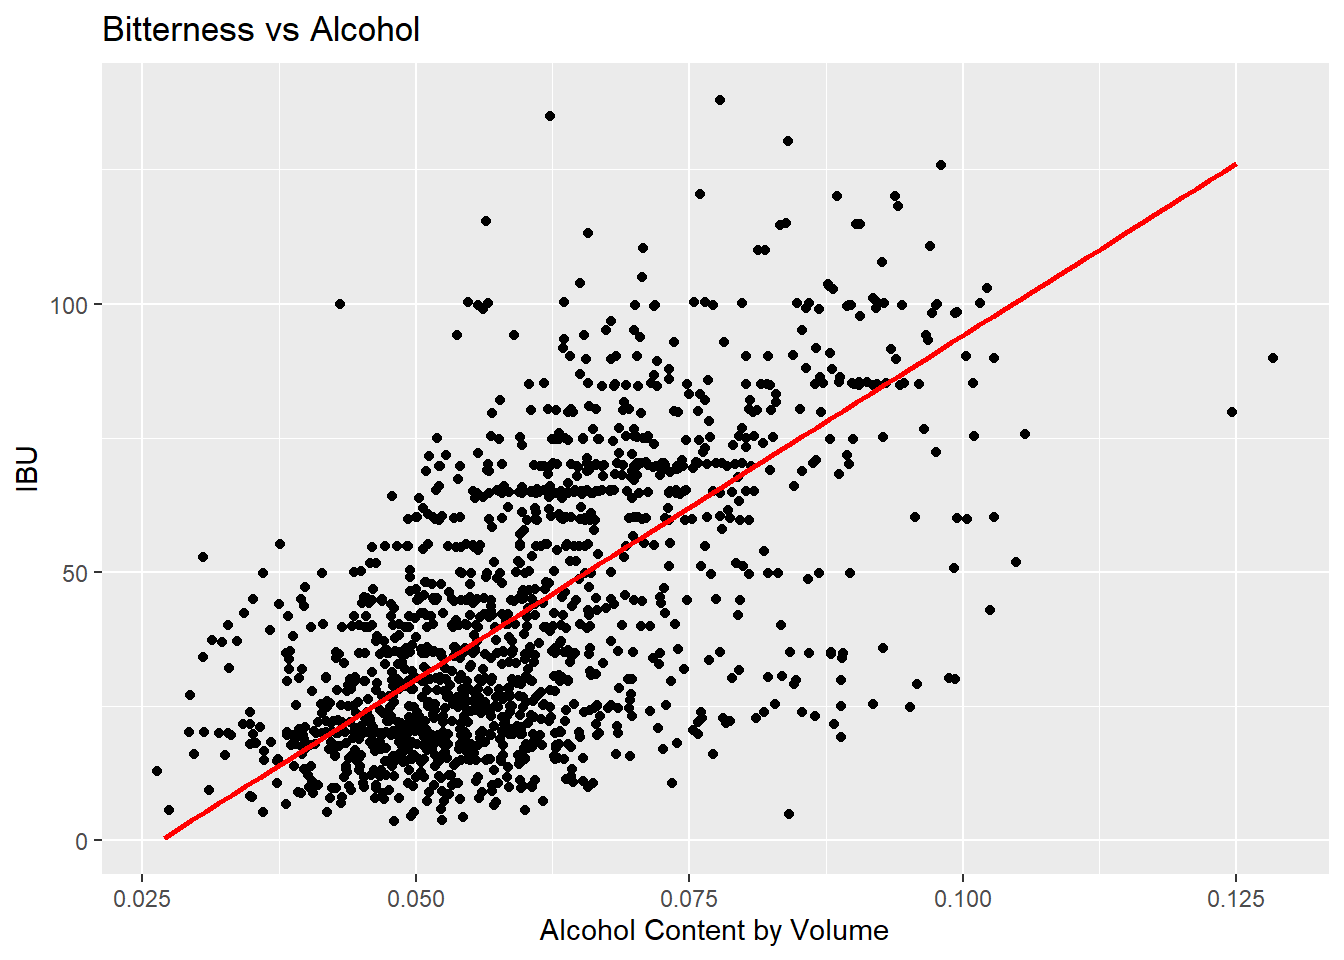
\includegraphics{CaseStudy2DDS_files/figure-latex/unnamed-chunk-8-1.pdf}

\begin{Shaded}
\begin{Highlighting}[]
\CommentTok{#grid.arrange(JL_plot, O_plot, JI_plot, JR_plot, MS_plot,}
\CommentTok{#  widths = c(1,1,1),c(1,1,1),layout_matrix = rbind(c(1, 2, 3))),c(4,5,5)))}
\NormalTok{df_chitest}
\end{Highlighting}
\end{Shaded}

\begin{verbatim}
##         Variable Chisq.pvalue
## 1       JobLevel 2.084703e-08
## 2       OverTime 2.332981e-15
## 3 JobInvolvement 5.211041e-09
## 4        JobRole 3.646836e-10
## 5  MaritalStatus 3.378946e-08
\end{verbatim}

\#\#NaiveBayes variables were:\\
* OverTime\\
* JobRole\\
* JobInvolvement\\
* MonthlyIncome\\
* TotalWorkingYears\\
* YearsInCurrentRole\\
* JobLevel

\begin{Shaded}
\begin{Highlighting}[]
\CommentTok{# Goal: reach a sensitivity and specificty greater than 60%}
\CommentTok{# add varables one by one until a desiered result is acheived}
\KeywordTok{set.seed}\NormalTok{(}\DecValTok{12}\NormalTok{)}
\NormalTok{splitPerc =}\StringTok{ }\FloatTok{.75}

\NormalTok{trainindex =}\StringTok{ }\KeywordTok{sample}\NormalTok{(}\KeywordTok{seq}\NormalTok{(}\DecValTok{1}\NormalTok{,}\KeywordTok{dim}\NormalTok{(data)[}\DecValTok{1}\NormalTok{],}\DecValTok{1}\NormalTok{), }\KeywordTok{round}\NormalTok{(splitPerc}\OperatorTok{*}\KeywordTok{dim}\NormalTok{(data)[}\DecValTok{1}\NormalTok{]))}

\NormalTok{trainIndices =}\StringTok{ }\KeywordTok{sample}\NormalTok{(}\KeywordTok{seq}\NormalTok{(}\DecValTok{1}\NormalTok{,}\KeywordTok{dim}\NormalTok{(data)[}\DecValTok{1}\NormalTok{],}\DecValTok{1}\NormalTok{),}\KeywordTok{round}\NormalTok{(splitPerc }\OperatorTok{*}\StringTok{ }\KeywordTok{dim}\NormalTok{(data)[}\DecValTok{1}\NormalTok{]))}
\NormalTok{train =}\StringTok{ }\NormalTok{data[trainindex,]}
\NormalTok{test =}\StringTok{ }\NormalTok{data[}\OperatorTok{-}\NormalTok{trainindex,]}
\CommentTok{#note it is illegal to know about relationship status when interviewing}

\NormalTok{m =}\StringTok{ }\KeywordTok{naiveBayes}\NormalTok{(Attrition}\OperatorTok{~}\NormalTok{OverTime}\OperatorTok{+}\NormalTok{JobRole}\OperatorTok{+}\NormalTok{JobInvolvement}\OperatorTok{+}\NormalTok{MonthlyIncome}\OperatorTok{+}\NormalTok{TotalWorkingYears}\OperatorTok{+}\NormalTok{JobLevel,}\DataTypeTok{data=}\NormalTok{train)}
\KeywordTok{table}\NormalTok{(}\KeywordTok{predict}\NormalTok{(m, }\DataTypeTok{newdata=}\NormalTok{test),test}\OperatorTok{$}\NormalTok{Attrition)}
\end{Highlighting}
\end{Shaded}

\begin{verbatim}
##      
##        No Yes
##   No  176  11
##   Yes  13  18
\end{verbatim}

\begin{Shaded}
\begin{Highlighting}[]
\NormalTok{CM =}\StringTok{ }\KeywordTok{confusionMatrix}\NormalTok{(}\KeywordTok{table}\NormalTok{(}\KeywordTok{predict}\NormalTok{(m, }\DataTypeTok{newdata=}\NormalTok{test),test}\OperatorTok{$}\NormalTok{Attrition))}
\NormalTok{CM}
\end{Highlighting}
\end{Shaded}

\begin{verbatim}
## Confusion Matrix and Statistics
## 
##      
##        No Yes
##   No  176  11
##   Yes  13  18
##                                           
##                Accuracy : 0.8899          
##                  95% CI : (0.8406, 0.9282)
##     No Information Rate : 0.867           
##     P-Value [Acc > NIR] : 0.1859          
##                                           
##                   Kappa : 0.5363          
##                                           
##  Mcnemar's Test P-Value : 0.8383          
##                                           
##             Sensitivity : 0.9312          
##             Specificity : 0.6207          
##          Pos Pred Value : 0.9412          
##          Neg Pred Value : 0.5806          
##              Prevalence : 0.8670          
##          Detection Rate : 0.8073          
##    Detection Prevalence : 0.8578          
##       Balanced Accuracy : 0.7760          
##                                           
##        'Positive' Class : No              
## 
\end{verbatim}

\begin{Shaded}
\begin{Highlighting}[]
\CommentTok{#grid.arrange(O_plot, JR_plot,JI_plot, mi_plot, twy_plot,yicr_plot,JL_plot)}

\NormalTok{comp_NB =}\StringTok{ }\KeywordTok{naiveBayes}\NormalTok{(Attrition}\OperatorTok{~}\NormalTok{OverTime}\OperatorTok{+}\NormalTok{MonthlyIncome}\OperatorTok{+}\NormalTok{JobRole}\OperatorTok{+}\NormalTok{TotalWorkingYears}\OperatorTok{+}\NormalTok{JobInvolvement}\OperatorTok{+}\NormalTok{JobLevel,}\DataTypeTok{data=}\NormalTok{data)}

\NormalTok{pred_att =}\StringTok{ }\KeywordTok{data.frame}\NormalTok{(}\DataTypeTok{Attrition =}\KeywordTok{predict}\NormalTok{(comp_NB, }\DataTypeTok{newdata=}\NormalTok{Comp_attr))}
\NormalTok{att_comp <-}\KeywordTok{bind_cols}\NormalTok{(Comp_attr,pred_att)}

\NormalTok{JR_plot}\OperatorTok{+}\StringTok{ }\NormalTok{(O_plot }\OperatorTok{+}\NormalTok{JI_plot)}\OperatorTok{+}\StringTok{ }\KeywordTok{plot_layout}\NormalTok{(}\DataTypeTok{ncol =} \DecValTok{1}\NormalTok{)}
\end{Highlighting}
\end{Shaded}

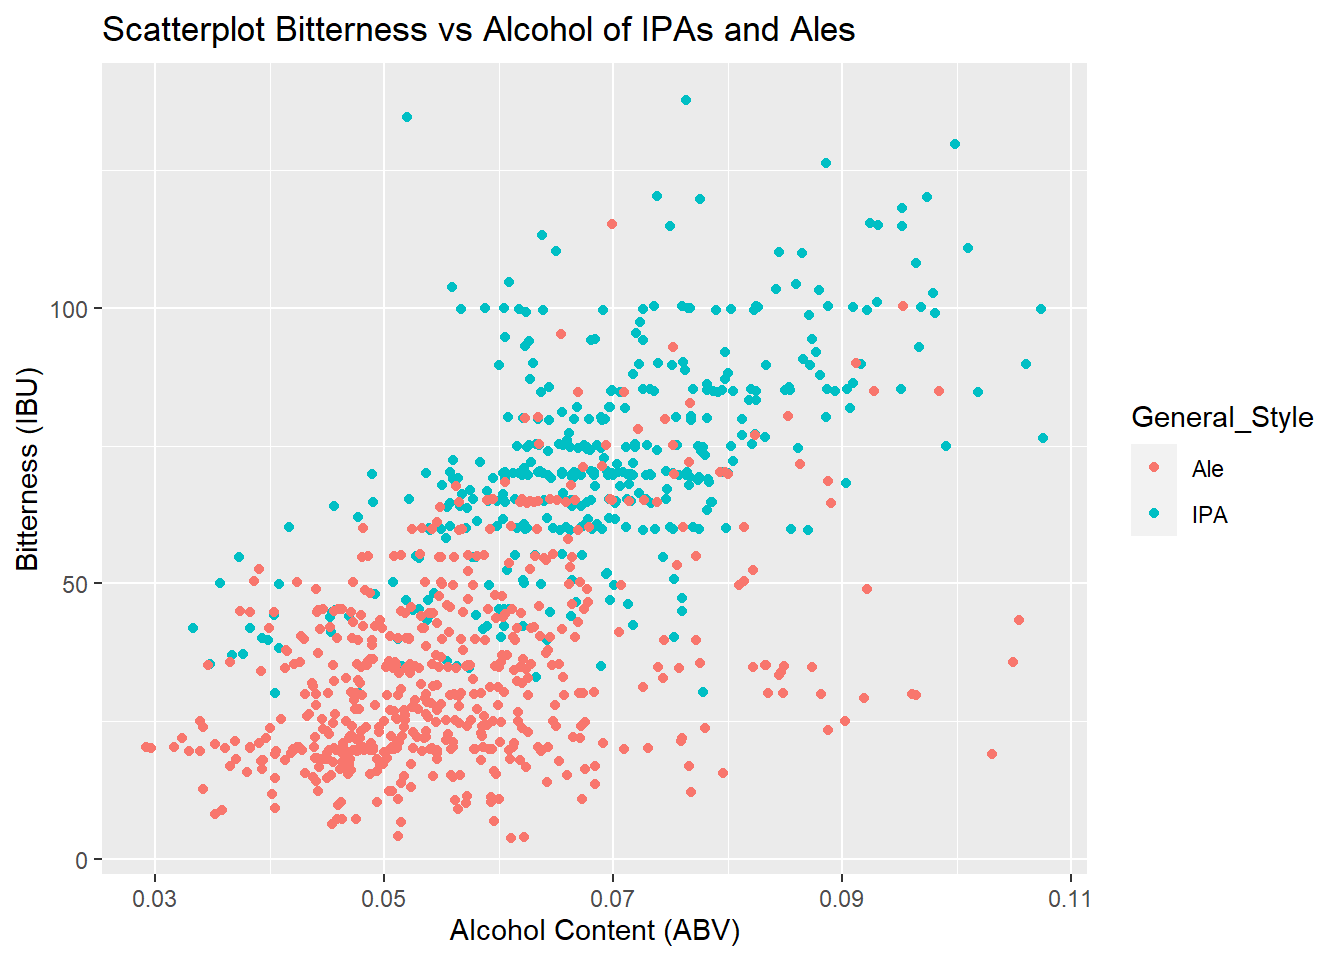
\includegraphics{CaseStudy2DDS_files/figure-latex/unnamed-chunk-9-1.pdf}

\begin{Shaded}
\begin{Highlighting}[]
\NormalTok{(mi_plot_box}\OperatorTok{+}\StringTok{ }\NormalTok{twy_plot_box)}\OperatorTok{+}\NormalTok{(JL_plot)}\OperatorTok{+}\StringTok{ }\KeywordTok{plot_layout}\NormalTok{(}\DataTypeTok{ncol =} \DecValTok{1}\NormalTok{)}
\end{Highlighting}
\end{Shaded}

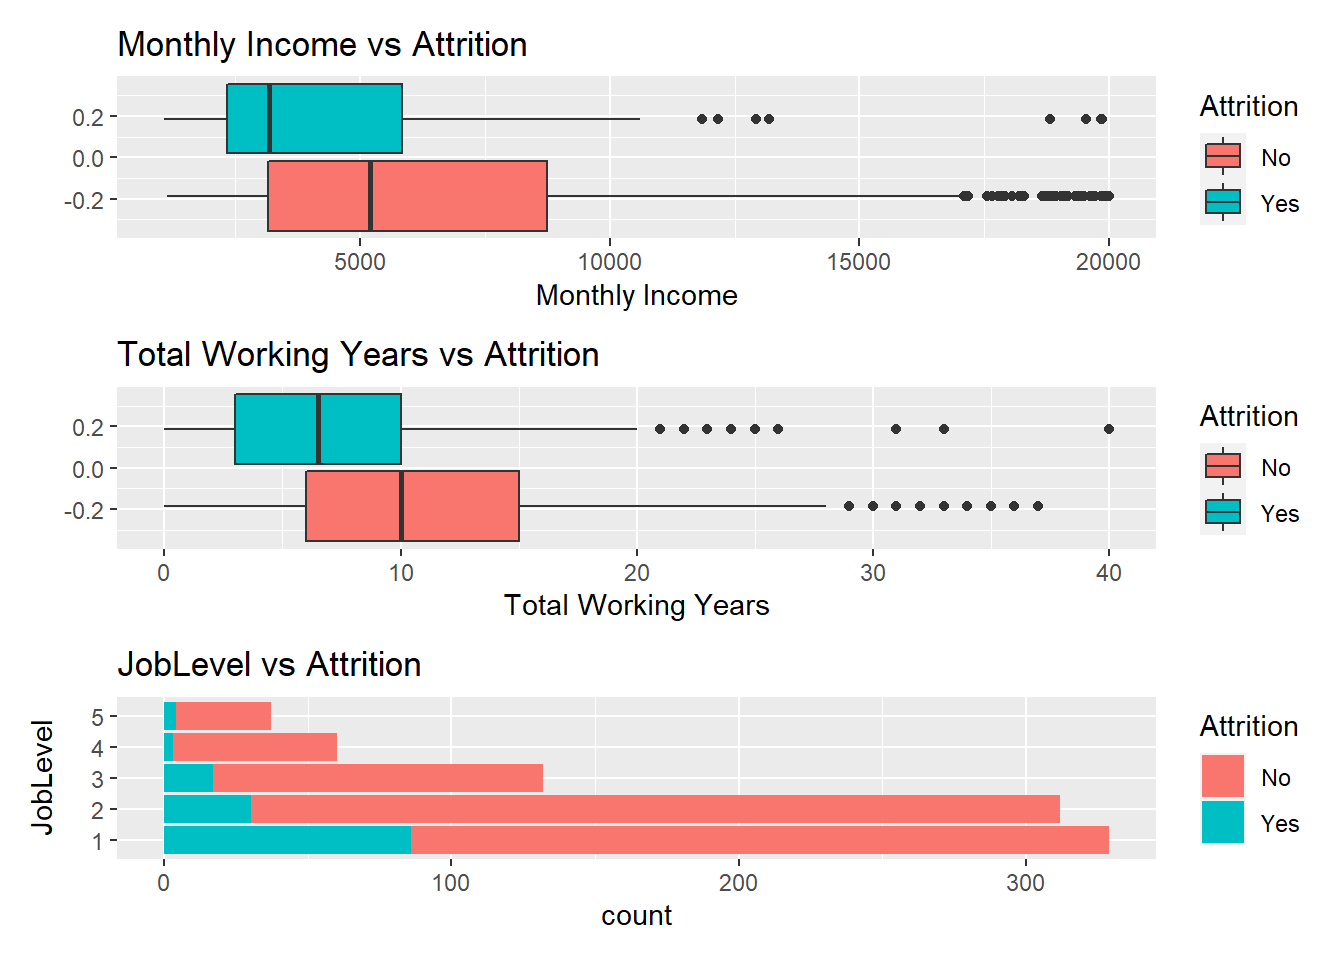
\includegraphics{CaseStudy2DDS_files/figure-latex/unnamed-chunk-9-2.pdf}

\begin{Shaded}
\begin{Highlighting}[]
\CommentTok{#this meets out goal but we could do better. It is dependent on the seed}
\CommentTok{#summary(att_comp)}


\CommentTok{#write.csv(select(att_comp,ID,Attrition),file="Case2Predictions_Scott_Attrition.csv")}
\end{Highlighting}
\end{Shaded}

\hypertarget{trying-a-better-model-could-be-overfitting-however.}{%
\subsection{trying a ``better model'' could be overfitting
however.}\label{trying-a-better-model-could-be-overfitting-however.}}

\begin{Shaded}
\begin{Highlighting}[]
\CommentTok{#Variables such as TotalWorkingYears, YearsAtCompany, YearsInCurrentRole, YearsSinceLastPromotion and YearsWithCurrentManager are highly corelated to each other.}
\CommentTok{# removed from the model due to colinearity. Left total working years}
\KeywordTok{set.seed}\NormalTok{(}\DecValTok{12}\NormalTok{)}
\NormalTok{splitPerc =}\StringTok{ }\FloatTok{.75}
\KeywordTok{head}\NormalTok{(data)}
\end{Highlighting}
\end{Shaded}

\begin{verbatim}
##   ID Age Attrition    BusinessTravel DailyRate             Department DistanceFromHome Education   EducationField
## 1  1  32        No     Travel_Rarely       117                  Sales               13         4    Life Sciences
## 2  2  40        No     Travel_Rarely      1308 Research & Development               14         3          Medical
## 3  3  35        No Travel_Frequently       200 Research & Development               18         2    Life Sciences
## 4  4  32        No     Travel_Rarely       801                  Sales                1         4        Marketing
## 5  5  24        No Travel_Frequently       567 Research & Development                2         1 Technical Degree
## 6  6  27        No Travel_Frequently       294 Research & Development               10         2    Life Sciences
##   EmployeeCount EmployeeNumber EnvironmentSatisfaction Gender HourlyRate JobInvolvement JobLevel
## 1             1            859                       2   Male         73              3        2
## 2             1           1128                       3   Male         44              2        5
## 3             1           1412                       3   Male         60              3        3
## 4             1           2016                       3 Female         48              3        3
## 5             1           1646                       1 Female         32              3        1
## 6             1            733                       4   Male         32              3        3
##                  JobRole JobSatisfaction MaritalStatus MonthlyIncome MonthlyRate NumCompaniesWorked Over18 OverTime
## 1        Sales Executive               4      Divorced          4403        9250                  2      Y       No
## 2      Research Director               3        Single         19626       17544                  1      Y       No
## 3 Manufacturing Director               4        Single          9362       19944                  2      Y       No
## 4        Sales Executive               4       Married         10422       24032                  1      Y       No
## 5     Research Scientist               4        Single          3760       17218                  1      Y      Yes
## 6 Manufacturing Director               1      Divorced          8793        4809                  1      Y       No
##   PercentSalaryHike PerformanceRating RelationshipSatisfaction StandardHours StockOptionLevel TotalWorkingYears
## 1                11                 3                        3            80                1                 8
## 2                14                 3                        1            80                0                21
## 3                11                 3                        3            80                0                10
## 4                19                 3                        3            80                2                14
## 5                13                 3                        3            80                0                 6
## 6                21                 4                        3            80                2                 9
##   TrainingTimesLastYear WorkLifeBalance YearsAtCompany YearsInCurrentRole YearsSinceLastPromotion
## 1                     3               2              5                  2                       0
## 2                     2               4             20                  7                       4
## 3                     2               3              2                  2                       2
## 4                     3               3             14                 10                       5
## 5                     2               3              6                  3                       1
## 6                     4               2              9                  7                       1
##   YearsWithCurrManager
## 1                    3
## 2                    9
## 3                    2
## 4                    7
## 5                    3
## 6                    7
\end{verbatim}

\begin{Shaded}
\begin{Highlighting}[]
\NormalTok{trainindex =}\StringTok{ }\KeywordTok{sample}\NormalTok{(}\KeywordTok{seq}\NormalTok{(}\DecValTok{1}\NormalTok{,}\KeywordTok{dim}\NormalTok{(data)[}\DecValTok{1}\NormalTok{],}\DecValTok{1}\NormalTok{), }\KeywordTok{round}\NormalTok{(splitPerc}\OperatorTok{*}\KeywordTok{dim}\NormalTok{(data)[}\DecValTok{1}\NormalTok{]))}

\NormalTok{trainIndices =}\StringTok{ }\KeywordTok{sample}\NormalTok{(}\KeywordTok{seq}\NormalTok{(}\DecValTok{1}\NormalTok{,}\KeywordTok{dim}\NormalTok{(data)[}\DecValTok{1}\NormalTok{],}\DecValTok{1}\NormalTok{),}\KeywordTok{round}\NormalTok{(splitPerc }\OperatorTok{*}\StringTok{ }\KeywordTok{dim}\NormalTok{(data)[}\DecValTok{1}\NormalTok{]))}
\NormalTok{train =}\StringTok{ }\NormalTok{data[trainindex,]}
\NormalTok{test =}\StringTok{ }\NormalTok{data[}\OperatorTok{-}\NormalTok{trainindex,]}
\CommentTok{#note it is illegal to know about relationship status when interviewing}
\NormalTok{m =}\StringTok{ }\KeywordTok{naiveBayes}\NormalTok{(Attrition}\OperatorTok{~}\NormalTok{BusinessTravel}\OperatorTok{+}\NormalTok{DistanceFromHome}\OperatorTok{+}\NormalTok{EnvironmentSatisfaction}\OperatorTok{+}\NormalTok{JobInvolvement}\OperatorTok{+}\NormalTok{JobSatisfaction}\OperatorTok{+}\NormalTok{MaritalStatus}\OperatorTok{+}\NormalTok{NumCompaniesWorked}\OperatorTok{+}\NormalTok{OverTime}\OperatorTok{+}\NormalTok{TotalWorkingYears}\OperatorTok{+}\NormalTok{RelationshipSatisfaction}\OperatorTok{+}\NormalTok{MonthlyIncome}\OperatorTok{+}\NormalTok{JobRole}\OperatorTok{+}\NormalTok{YearsInCurrentRole}\OperatorTok{+}\NormalTok{JobLevel,}\DataTypeTok{data=}\NormalTok{train)}
\KeywordTok{table}\NormalTok{(}\KeywordTok{predict}\NormalTok{(m, }\DataTypeTok{newdata=}\NormalTok{test),test}\OperatorTok{$}\NormalTok{Attrition)}
\end{Highlighting}
\end{Shaded}

\begin{verbatim}
##      
##        No Yes
##   No  168  10
##   Yes  21  19
\end{verbatim}

\begin{Shaded}
\begin{Highlighting}[]
\NormalTok{CM =}\StringTok{ }\KeywordTok{confusionMatrix}\NormalTok{(}\KeywordTok{table}\NormalTok{(}\KeywordTok{predict}\NormalTok{(m, }\DataTypeTok{newdata=}\NormalTok{test),test}\OperatorTok{$}\NormalTok{Attrition))}
\NormalTok{CM}
\end{Highlighting}
\end{Shaded}

\begin{verbatim}
## Confusion Matrix and Statistics
## 
##      
##        No Yes
##   No  168  10
##   Yes  21  19
##                                           
##                Accuracy : 0.8578          
##                  95% CI : (0.8043, 0.9013)
##     No Information Rate : 0.867           
##     P-Value [Acc > NIR] : 0.69734         
##                                           
##                   Kappa : 0.4688          
##                                           
##  Mcnemar's Test P-Value : 0.07249         
##                                           
##             Sensitivity : 0.8889          
##             Specificity : 0.6552          
##          Pos Pred Value : 0.9438          
##          Neg Pred Value : 0.4750          
##              Prevalence : 0.8670          
##          Detection Rate : 0.7706          
##    Detection Prevalence : 0.8165          
##       Balanced Accuracy : 0.7720          
##                                           
##        'Positive' Class : No              
## 
\end{verbatim}

\begin{Shaded}
\begin{Highlighting}[]
\CommentTok{#grid.arrange(O_plot, JR_plot,JI_plot, mi_plot, twy_plot,yicr_plot,JL_plot)}

\NormalTok{comp_NB =}\StringTok{ }\KeywordTok{naiveBayes}\NormalTok{(Attrition}\OperatorTok{~}\NormalTok{BusinessTravel}\OperatorTok{+}\NormalTok{DistanceFromHome}\OperatorTok{+}\NormalTok{EnvironmentSatisfaction}\OperatorTok{+}\NormalTok{JobInvolvement}\OperatorTok{+}\NormalTok{JobSatisfaction}\OperatorTok{+}\NormalTok{MaritalStatus}\OperatorTok{+}\NormalTok{NumCompaniesWorked}\OperatorTok{+}\NormalTok{OverTime}\OperatorTok{+}\NormalTok{TotalWorkingYears}\OperatorTok{+}\NormalTok{RelationshipSatisfaction}\OperatorTok{+}\NormalTok{MonthlyIncome}\OperatorTok{+}\NormalTok{JobRole}\OperatorTok{+}\NormalTok{YearsInCurrentRole}\OperatorTok{+}\NormalTok{JobLevel,}\DataTypeTok{data=}\NormalTok{data)}

\NormalTok{pred_att =}\StringTok{ }\KeywordTok{data.frame}\NormalTok{(}\DataTypeTok{Attrition =}\KeywordTok{predict}\NormalTok{(comp_NB, }\DataTypeTok{newdata=}\NormalTok{Comp_attr))}
\NormalTok{att_comp <-}\KeywordTok{bind_cols}\NormalTok{(Comp_attr,pred_att)}
\end{Highlighting}
\end{Shaded}

\hypertarget{salary-eda}{%
\subsection{Salary EDA}\label{salary-eda}}

Categorical Variables Vs MonthlyIncome * JobLevel\\
* Education\\
* JobRole\\
* EducationField

\begin{Shaded}
\begin{Highlighting}[]
\CommentTok{#Ordinal variable EDA}
\CommentTok{#data %>% select(Education, EnvironmentSatisfaction, JobInvolvement, JobSatisfaction, PerformanceRating, WorkLifeBalance, JobLevel, RelationshipSatisfaction, MonthlyIncome) %>% ggpairs(upper = list(continuous="smooth", combo="box", discrete = "facetbar"), lower=list(continuous="smooth", combo="box", discrete = "facetbar"))}
\CommentTok{# Correlation to JobLevel, maybe Education}

\NormalTok{JLS_plot <-}\StringTok{ }\NormalTok{data }\OperatorTok\StringTok{ }\KeywordTok{ggplot}\NormalTok{(}\KeywordTok{aes}\NormalTok{(JobLevel, MonthlyIncome))}\OperatorTok{+}\KeywordTok{geom_boxplot}\NormalTok{()}\OperatorTok{+}\KeywordTok{labs}\NormalTok{(}\DataTypeTok{title=}\StringTok{"Job Level vs MI"}\NormalTok{)}

\NormalTok{ES_plot <-}\StringTok{ }\NormalTok{data }\OperatorTok\StringTok{ }\KeywordTok{ggplot}\NormalTok{(}\KeywordTok{aes}\NormalTok{(Education, MonthlyIncome))}\OperatorTok{+}\KeywordTok{geom_boxplot}\NormalTok{()}\OperatorTok{+}\KeywordTok{labs}\NormalTok{(}\DataTypeTok{title=}\StringTok{"Education vs MI"}\NormalTok{)}

\CommentTok{#Nominal variable EDA}
\CommentTok{#data %>% select(Attrition, BusinessTravel, Department, EducationField, Gender, JobRole, MaritalStatus, OverTime, MonthlyIncome) %>% ggpairs(upper = list(continuous="smooth", combo="box", discrete = "facetbar"), lower=list(continuous="smooth", combo="box", discrete = "facetbar"))}
\CommentTok{# JobRole has interesting differences.  Maybe EducationField}

\NormalTok{JRS_plot <-}\StringTok{ }\NormalTok{data }\OperatorTok\StringTok{ }\KeywordTok{ggplot}\NormalTok{(}\KeywordTok{aes}\NormalTok{(JobRole,MonthlyIncome))}\OperatorTok{+}\KeywordTok{geom_boxplot}\NormalTok{()}\OperatorTok{+}\KeywordTok{labs}\NormalTok{(}\DataTypeTok{title=}\StringTok{"Job Role vs MI"}\NormalTok{)}\OperatorTok{+}\KeywordTok{coord_flip}\NormalTok{()}

\NormalTok{EFS_plot <-}\StringTok{ }\NormalTok{data }\OperatorTok\StringTok{ }\KeywordTok{ggplot}\NormalTok{(}\KeywordTok{aes}\NormalTok{(EducationField,MonthlyIncome))}\OperatorTok{+}\KeywordTok{geom_boxplot}\NormalTok{()}\OperatorTok{+}\KeywordTok{labs}\NormalTok{(}\DataTypeTok{title=}\StringTok{"Education Field vs MI"}\NormalTok{)}\OperatorTok{+}\KeywordTok{coord_flip}\NormalTok{()}

\NormalTok{JLS_plot}\OperatorTok{+}\NormalTok{EFS_plot}\OperatorTok{+}\StringTok{ }\NormalTok{ES_plot }\OperatorTok{+}\StringTok{ }\NormalTok{JRS_plot}\OperatorTok{+}\StringTok{  }\KeywordTok{plot_layout}\NormalTok{(}\DataTypeTok{ncol =} \DecValTok{2}\NormalTok{)}
\end{Highlighting}
\end{Shaded}

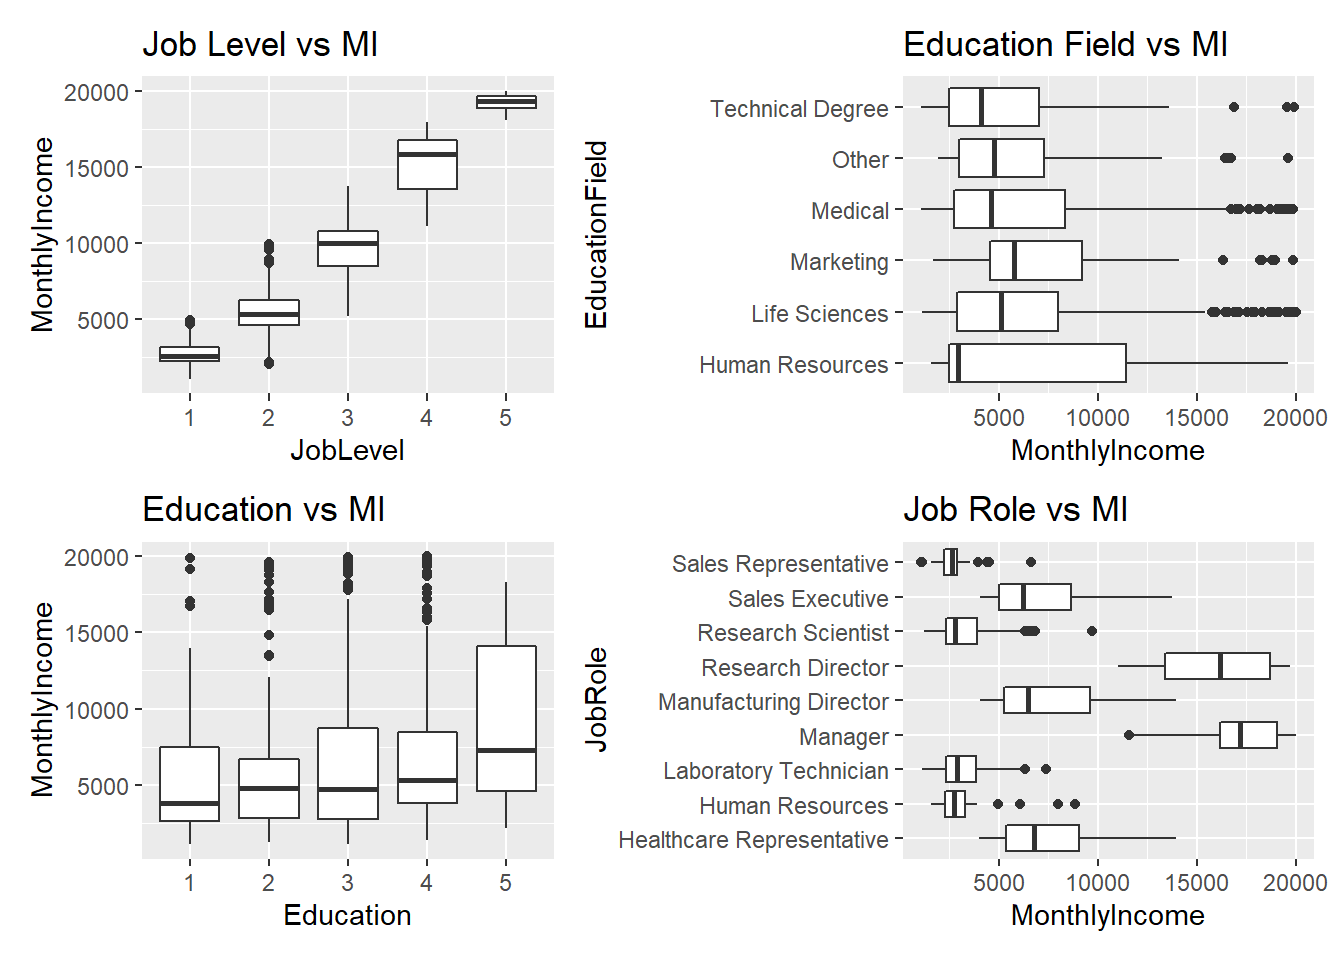
\includegraphics{CaseStudy2DDS_files/figure-latex/unnamed-chunk-11-1.pdf}

\begin{Shaded}
\begin{Highlighting}[]
\CommentTok{#grid.arrange(JLS_plot, ES_plot, JRS_plot, EFS_plot)}
\end{Highlighting}
\end{Shaded}

\hypertarget{continious-varables}{%
\subsection{Continious Varables}\label{continious-varables}}

\begin{itemize}
\tightlist
\item
  Age\\
\item
  TotalWorkingYears\\
\item
  Years at Company
\end{itemize}

\begin{Shaded}
\begin{Highlighting}[]
\CommentTok{# there is a possibility that total years worked and years at company could be colinear and we do not want that}

\CommentTok{#Continous variable EDA}
\CommentTok{#data %>% select(Age,DailyRate, DistanceFromHome, HourlyRate, MonthlyRate, NumCompaniesWorked, PercentSalaryHike, MonthlyIncome) %>% ggpairs(upper = list(continuous="smooth", combo="box", discrete = "facetbar"), lower=list(continuous="smooth", combo="box", discrete = "facetbar"))}
\CommentTok{# Age has a positive correlation}

\NormalTok{AgS_plot <-}\StringTok{ }\NormalTok{data }\OperatorTok\StringTok{ }\KeywordTok{ggplot}\NormalTok{(}\KeywordTok{aes}\NormalTok{(Age,MonthlyIncome))}\OperatorTok{+}\KeywordTok{geom_point}\NormalTok{()}\OperatorTok{+}\KeywordTok{geom_smooth}\NormalTok{(}\DataTypeTok{method=}\StringTok{"lm"}\NormalTok{)}\OperatorTok{+}\KeywordTok{labs}\NormalTok{(}\DataTypeTok{title =} \StringTok{"Age vs Monthly Income"}\NormalTok{)}

\CommentTok{#data %>% select(StockOptionLevel, TotalWorkingYears, TrainingTimesLastYear, YearsSinceLastPromotion, YearsInCurrentRole, YearsWithCurrManager, YearsAtCompany, MonthlyIncome) %>% ggpairs(upper = list(continuous="smooth", combo="box", discrete = "facetbar"), lower=list(continuous="smooth", combo="box", discrete = "facetbar"))}
\CommentTok{#TotalWorking Years and YearsatCompany have a strong correlation}
\CommentTok{#Years SinceLastPromotion, InCurrentRole and WithCurrManager have weak positive correlation}

\NormalTok{TWYS_plot <-}\StringTok{ }\NormalTok{data }\OperatorTok\StringTok{ }\KeywordTok{ggplot}\NormalTok{(}\KeywordTok{aes}\NormalTok{(TotalWorkingYears,MonthlyIncome))}\OperatorTok{+}\KeywordTok{geom_point}\NormalTok{()}\OperatorTok{+}\KeywordTok{geom_smooth}\NormalTok{(}\DataTypeTok{method=}\StringTok{"lm"}\NormalTok{)}\OperatorTok{+}\KeywordTok{labs}\NormalTok{(}\DataTypeTok{title =} \StringTok{"TotalWorkingYears vs Monthly Income"}\NormalTok{)}

\NormalTok{YaCS_plot <-}\StringTok{ }\NormalTok{data }\OperatorTok\StringTok{ }\KeywordTok{ggplot}\NormalTok{(}\KeywordTok{aes}\NormalTok{(YearsAtCompany,MonthlyIncome))}\OperatorTok{+}\KeywordTok{geom_point}\NormalTok{()}\OperatorTok{+}\KeywordTok{geom_smooth}\NormalTok{(}\DataTypeTok{method=}\StringTok{"lm"}\NormalTok{)}\OperatorTok{+}\KeywordTok{labs}\NormalTok{(}\DataTypeTok{title =} \StringTok{"YearsAtCompany vs Monthly Income"}\NormalTok{)}

\KeywordTok{grid.arrange}\NormalTok{(AgS_plot,TWYS_plot, YaCS_plot)}
\end{Highlighting}
\end{Shaded}

\begin{verbatim}
## `geom_smooth()` using formula 'y ~ x'
## `geom_smooth()` using formula 'y ~ x'
## `geom_smooth()` using formula 'y ~ x'
\end{verbatim}

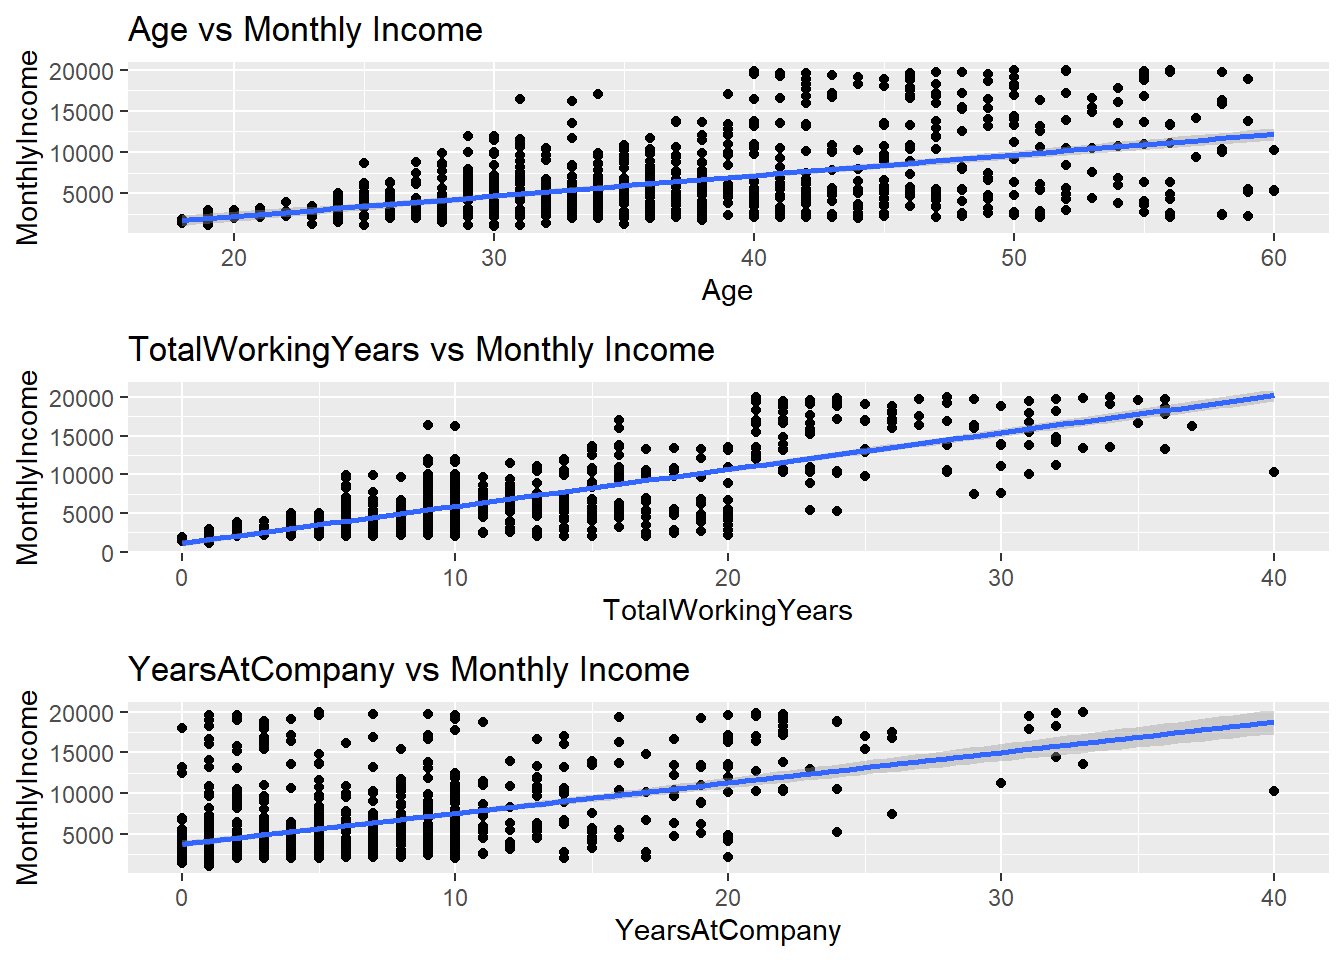
\includegraphics{CaseStudy2DDS_files/figure-latex/unnamed-chunk-12-1.pdf}

\begin{Shaded}
\begin{Highlighting}[]
\NormalTok{corr_data <-}\StringTok{ }\NormalTok{data }\OperatorTok\StringTok{ }\KeywordTok{select}\NormalTok{(Age, TotalWorkingYears, YearsAtCompany, YearsSinceLastPromotion, YearsInCurrentRole, YearsWithCurrManager, MonthlyIncome)}

\NormalTok{corr <-}\StringTok{ }\KeywordTok{round}\NormalTok{(}\KeywordTok{cor}\NormalTok{(corr_data),}\DecValTok{1}\NormalTok{)}

\KeywordTok{ggcorrplot}\NormalTok{(corr, }\DataTypeTok{hc.order =} \OtherTok{TRUE}\NormalTok{, }
           \DataTypeTok{type =} \StringTok{"lower"}\NormalTok{, }
           \DataTypeTok{lab =} \OtherTok{TRUE}\NormalTok{, }
           \DataTypeTok{lab_size =} \DecValTok{3}\NormalTok{, }
           \DataTypeTok{method=}\StringTok{"circle"}\NormalTok{, }
           \DataTypeTok{colors =} \KeywordTok{c}\NormalTok{(}\StringTok{"red"}\NormalTok{, }\StringTok{"white"}\NormalTok{, }\StringTok{"springgreen3"}\NormalTok{), }
           \DataTypeTok{title=}\StringTok{"Correlogram of Continuous Variables"}\NormalTok{, }
           \DataTypeTok{ggtheme=}\NormalTok{theme_bw)}
\end{Highlighting}
\end{Shaded}

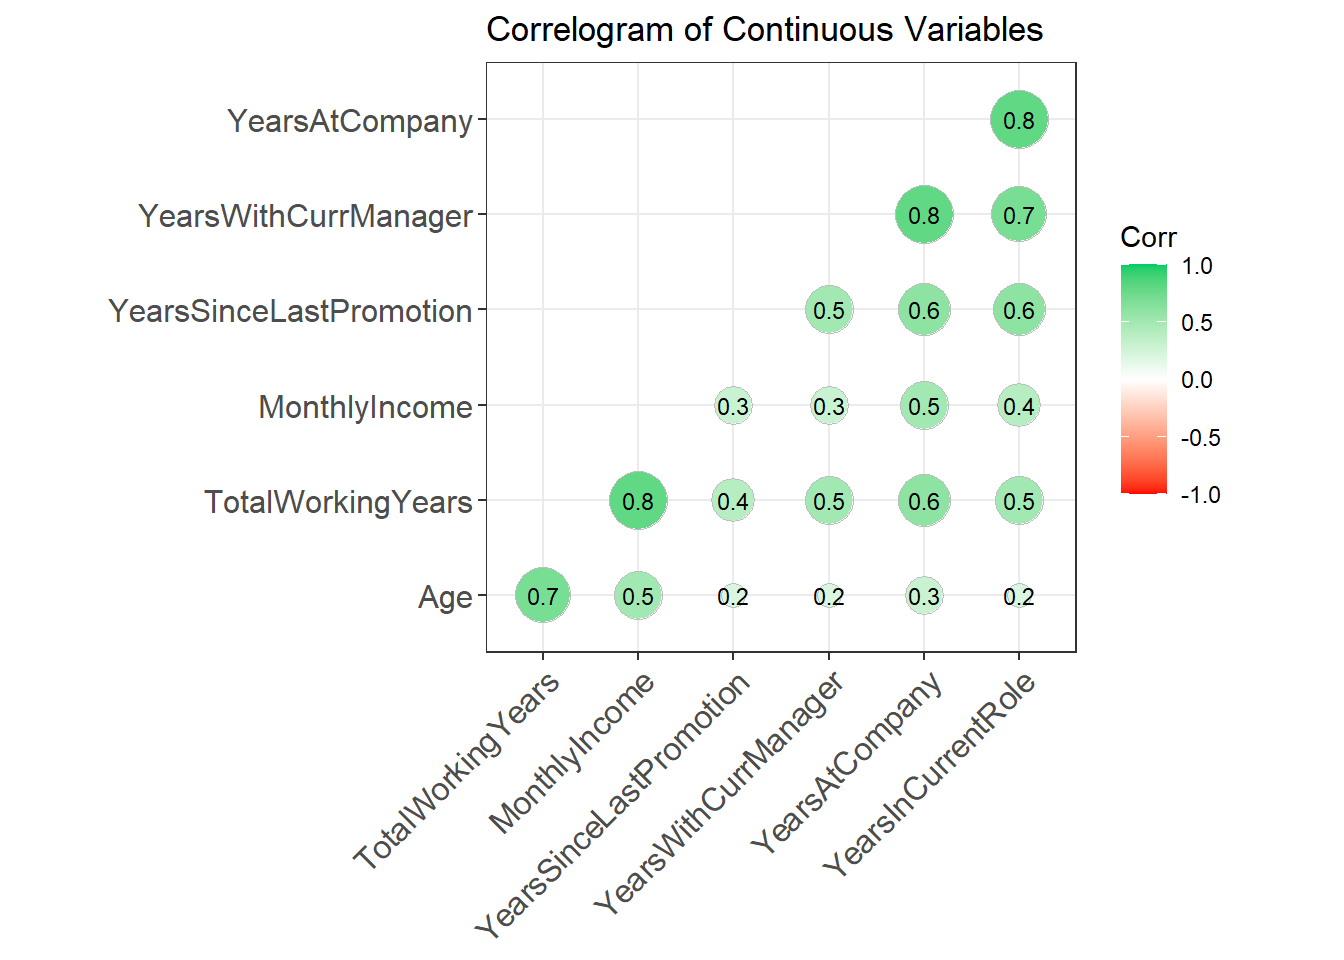
\includegraphics{CaseStudy2DDS_files/figure-latex/unnamed-chunk-12-2.pdf}

\hypertarget{lm-salary}{%
\subsection{LM Salary}\label{lm-salary}}

\begin{Shaded}
\begin{Highlighting}[]
\NormalTok{Salary_train <-}\StringTok{ }\NormalTok{data }\OperatorTok\StringTok{ }\KeywordTok{select}\NormalTok{(MonthlyIncome, TotalWorkingYears, JobLevel)}

\NormalTok{fit <-}\StringTok{ }\KeywordTok{lm}\NormalTok{(MonthlyIncome}\OperatorTok{~}\NormalTok{TotalWorkingYears}\OperatorTok{+}\NormalTok{JobLevel, }\DataTypeTok{data=}\NormalTok{Salary_train)}

\KeywordTok{summary}\NormalTok{(fit)}
\end{Highlighting}
\end{Shaded}

\begin{verbatim}
## 
## Call:
## lm(formula = MonthlyIncome ~ TotalWorkingYears + JobLevel, data = Salary_train)
## 
## Residuals:
##     Min      1Q  Median      3Q     Max 
## -4957.9  -657.8  -134.6   618.2  4525.8 
## 
## Coefficients:
##                    Estimate Std. Error t value Pr(>|t|)    
## (Intercept)        2544.901     89.085  28.567  < 2e-16 ***
## TotalWorkingYears    33.442      9.426   3.548 0.000409 ***
## JobLevel2          2652.205    107.666  24.634  < 2e-16 ***
## JobLevel3          6820.371    152.732  44.656  < 2e-16 ***
## JobLevel4         11858.212    254.564  46.582  < 2e-16 ***
## JobLevel5         15800.546    289.997  54.485  < 2e-16 ***
## ---
## Signif. codes:  0 '***' 0.001 '**' 0.01 '*' 0.05 '.' 0.1 ' ' 1
## 
## Residual standard error: 1256 on 864 degrees of freedom
## Multiple R-squared:  0.9258, Adjusted R-squared:  0.9254 
## F-statistic:  2157 on 5 and 864 DF,  p-value: < 2.2e-16
\end{verbatim}

\begin{Shaded}
\begin{Highlighting}[]
\CommentTok{#confint(fit)}

\KeywordTok{train}\NormalTok{(MonthlyIncome}\OperatorTok{~}\NormalTok{TotalWorkingYears}\OperatorTok{+}\NormalTok{JobLevel, }\DataTypeTok{method=}\StringTok{"lm"}\NormalTok{,}\DataTypeTok{data=}\NormalTok{Salary_train, }\DataTypeTok{trControl =} \KeywordTok{trainControl}\NormalTok{(}\DataTypeTok{method =} \StringTok{"LOOCV"}\NormalTok{))}
\end{Highlighting}
\end{Shaded}

\begin{verbatim}
## Linear Regression 
## 
## 870 samples
##   2 predictor
## 
## No pre-processing
## Resampling: Leave-One-Out Cross-Validation 
## Summary of sample sizes: 869, 869, 869, 869, 869, 869, ... 
## Resampling results:
## 
##   RMSE      Rsquared   MAE     
##   1261.666  0.9246115  915.7436
## 
## Tuning parameter 'intercept' was held constant at a value of TRUE
\end{verbatim}

\begin{Shaded}
\begin{Highlighting}[]
\KeywordTok{grid.arrange}\NormalTok{(TWYS_plot, JLS_plot)}
\end{Highlighting}
\end{Shaded}

\begin{verbatim}
## `geom_smooth()` using formula 'y ~ x'
\end{verbatim}

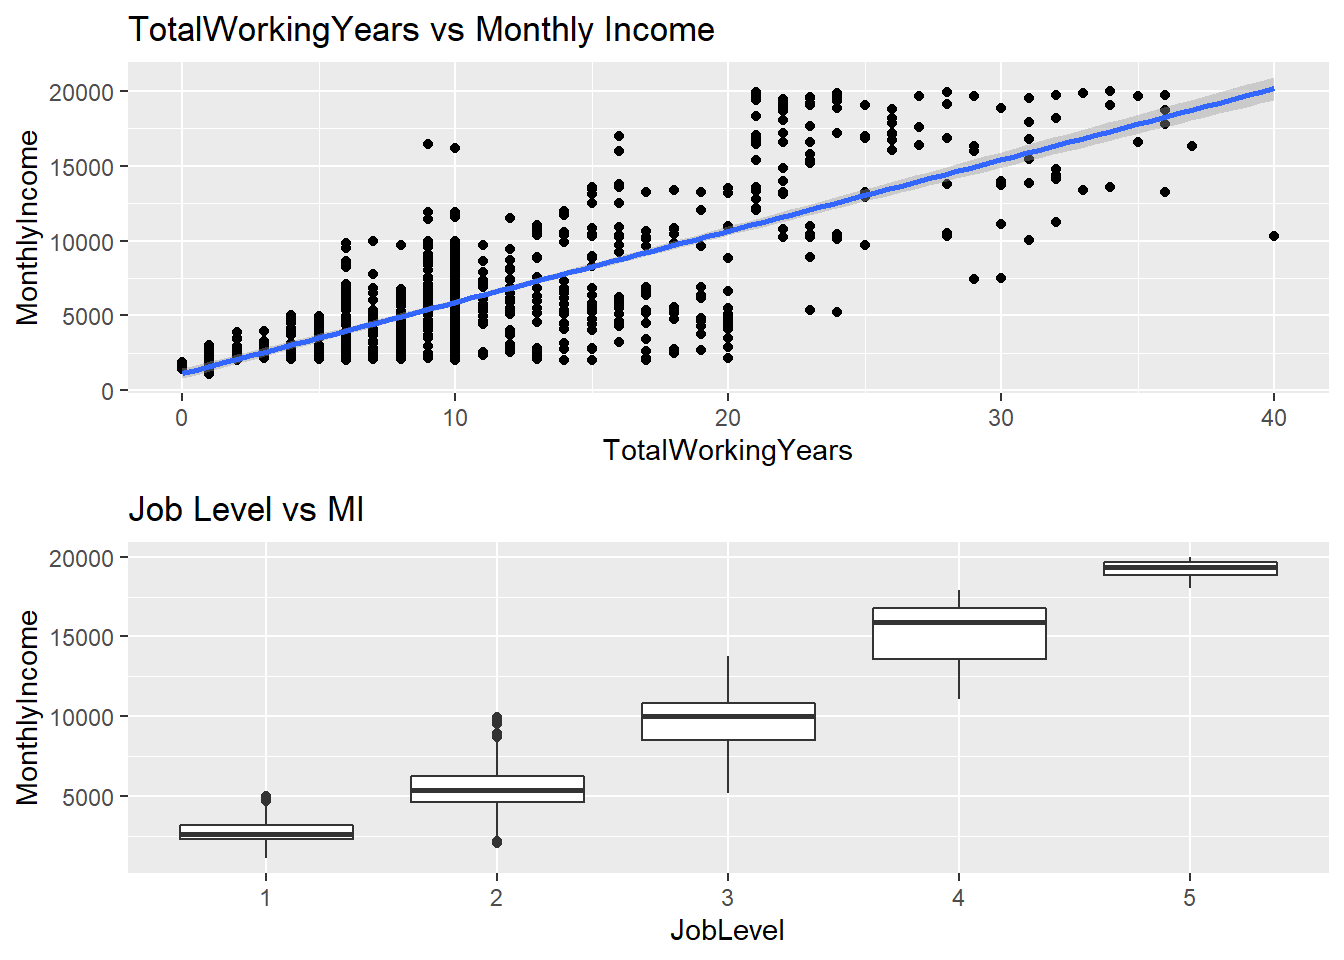
\includegraphics{CaseStudy2DDS_files/figure-latex/unnamed-chunk-13-1.pdf}

\begin{Shaded}
\begin{Highlighting}[]
\NormalTok{pred_sal =}\StringTok{ }\KeywordTok{data.frame}\NormalTok{(}\DataTypeTok{MonthlyIncome =} \KeywordTok{predict}\NormalTok{(fit, }\DataTypeTok{newdata =}\NormalTok{ Comp_sal))}
\NormalTok{sal_comp <-}\KeywordTok{bind_cols}\NormalTok{(Comp_sal, pred_sal)}

\CommentTok{#summary(sal_comp)}

\CommentTok{#write.csv(select(sal_comp,ID,MonthlyIncome), file="Case2Predictions_Scott_Salary.csv")}
\end{Highlighting}
\end{Shaded}

\end{document}
